\documentclass[11pt,a4paper]{article}

% ============================================================
%  QIMMA -- POLYCOPIÉ : Mathématiques — 2ème Bac Sciences Maths
%  Assemble les PDF des chapitres (compiler d'abord chaque
%  chapitre : make matiere DIR=cours/bac2/sciences-maths/mathematiques)
% ============================================================

\usepackage[a4paper,margin=0cm]{geometry}
\usepackage{pdfpages}

\begin{document}

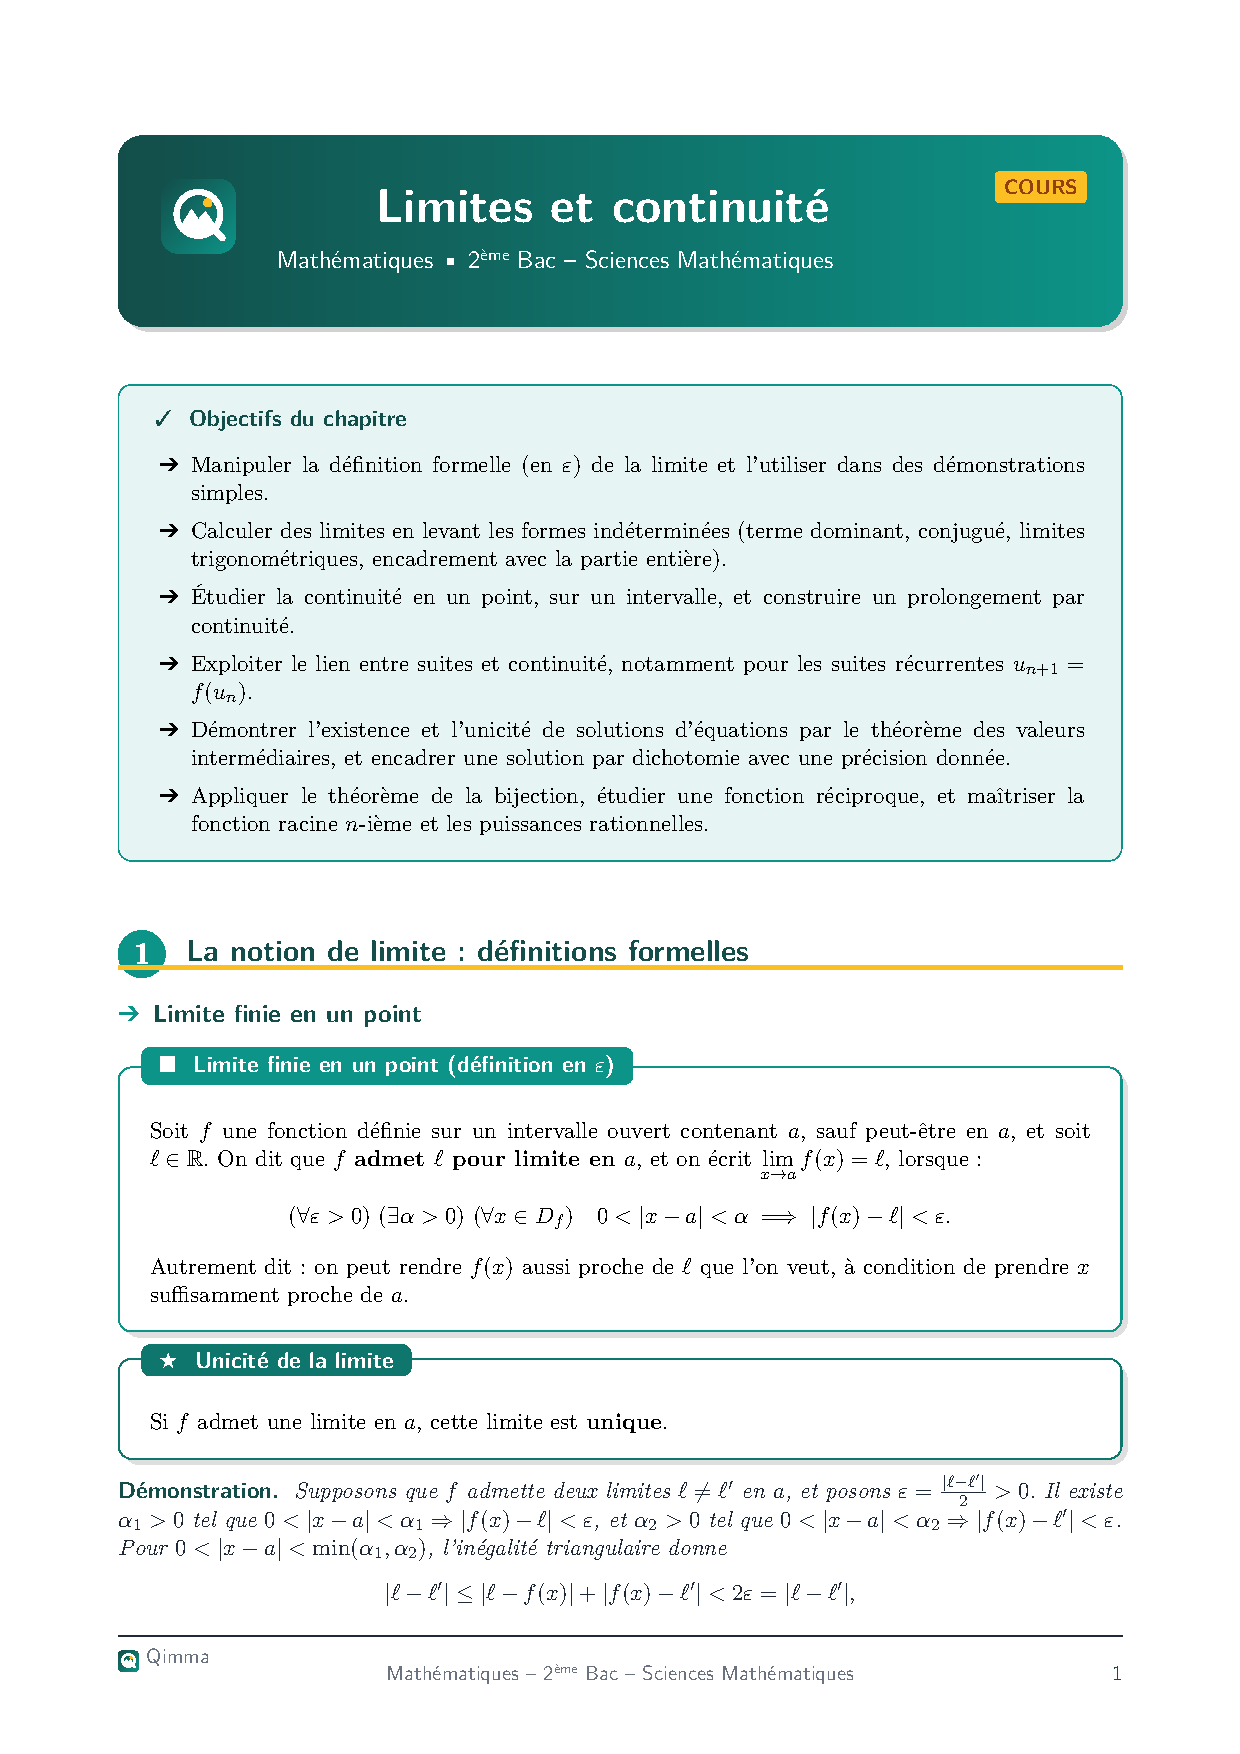
\includepdf[pages=-]{01-limites-et-continuite.pdf}
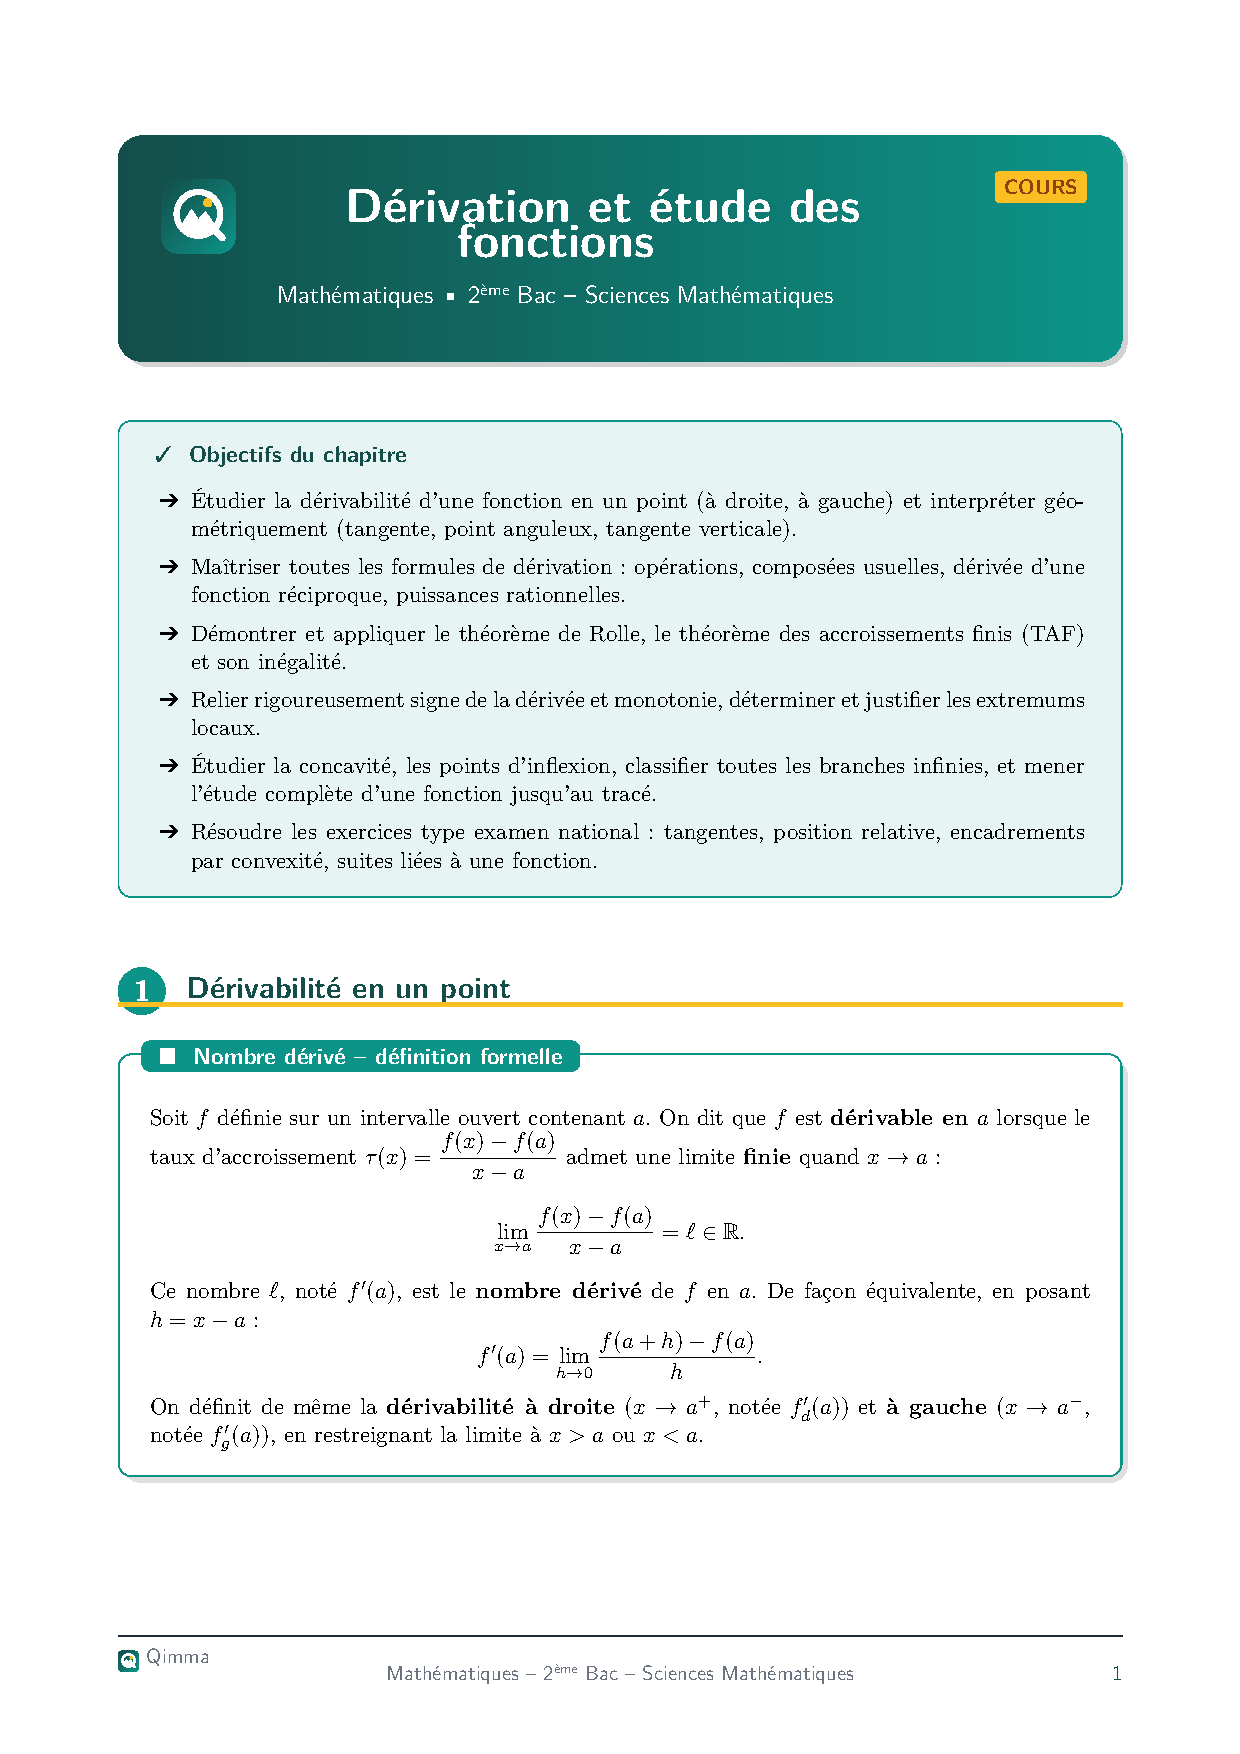
\includepdf[pages=-]{02-derivation-et-etude-des-fonctions.pdf}
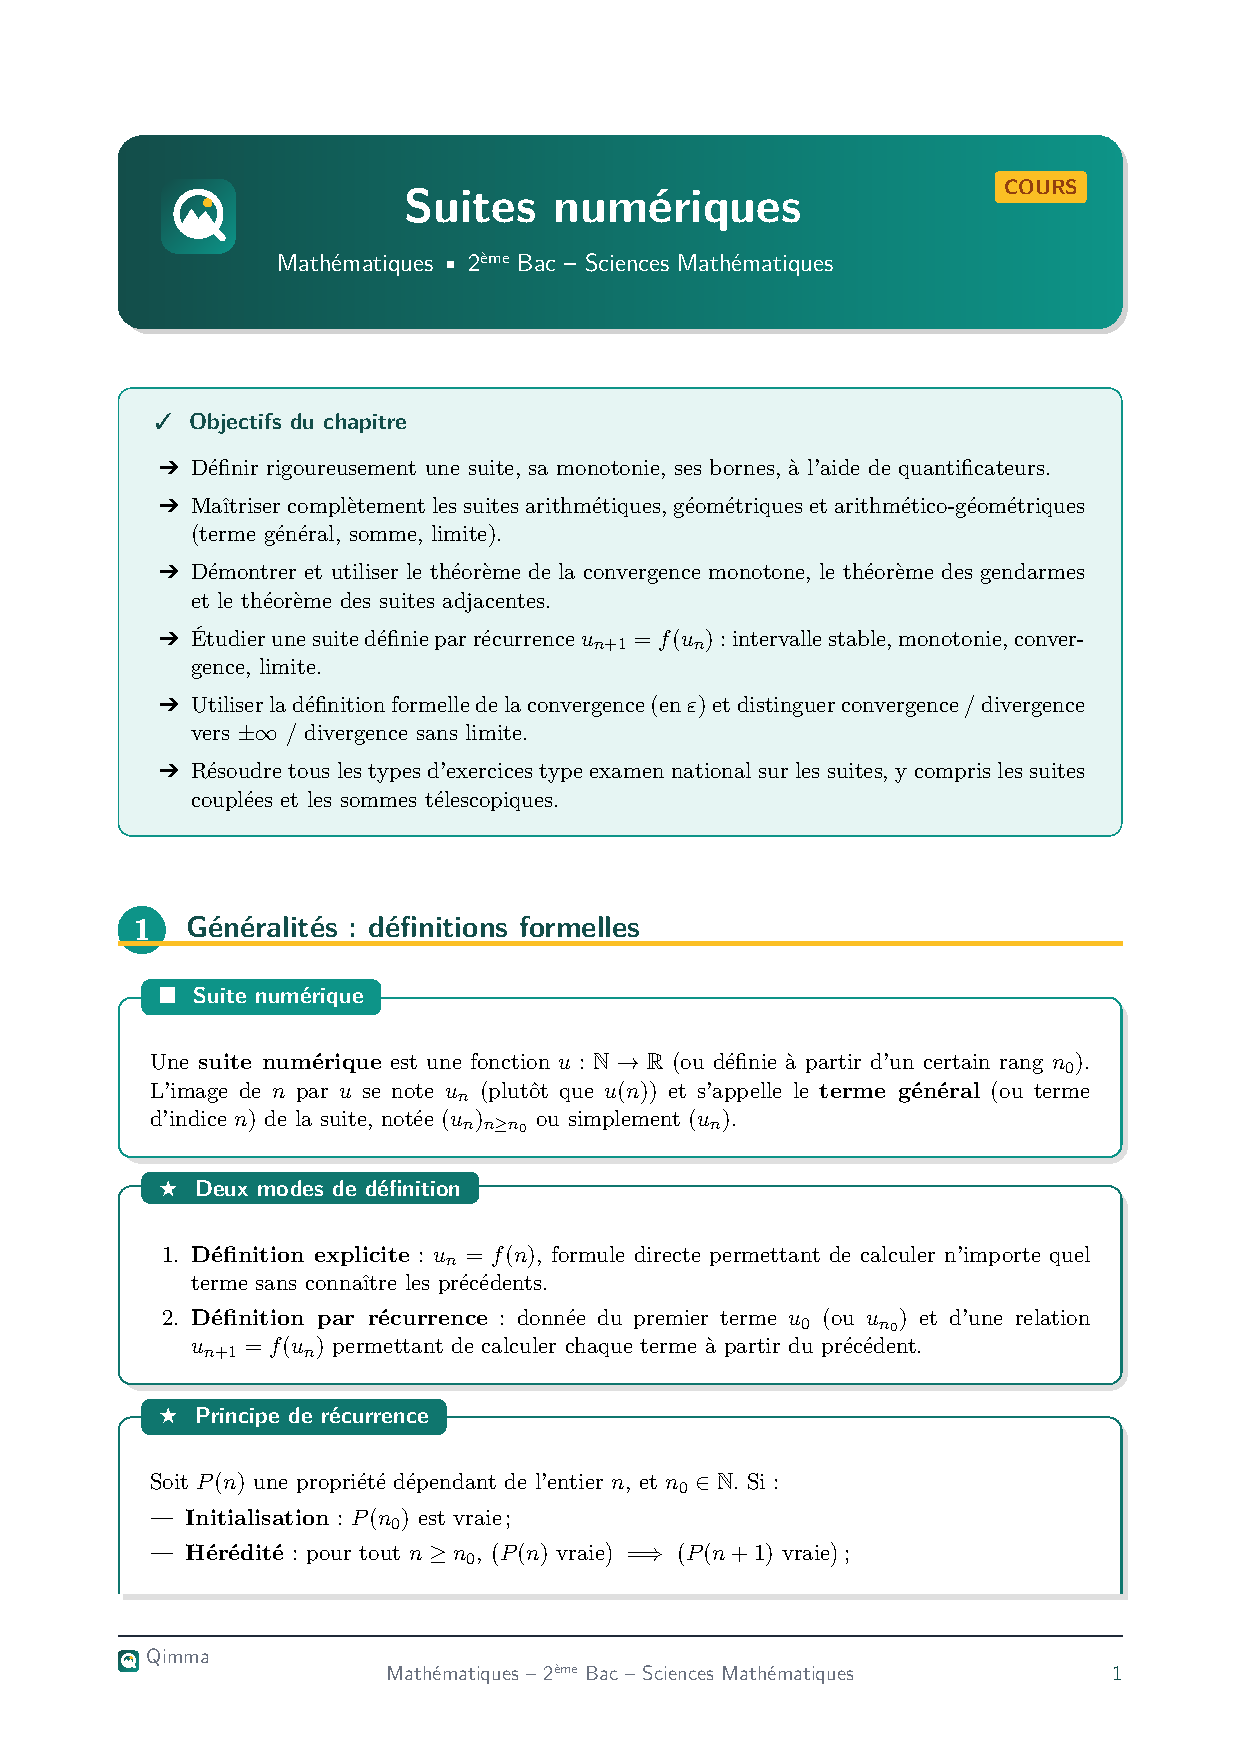
\includepdf[pages=-]{03-suites-numeriques.pdf}
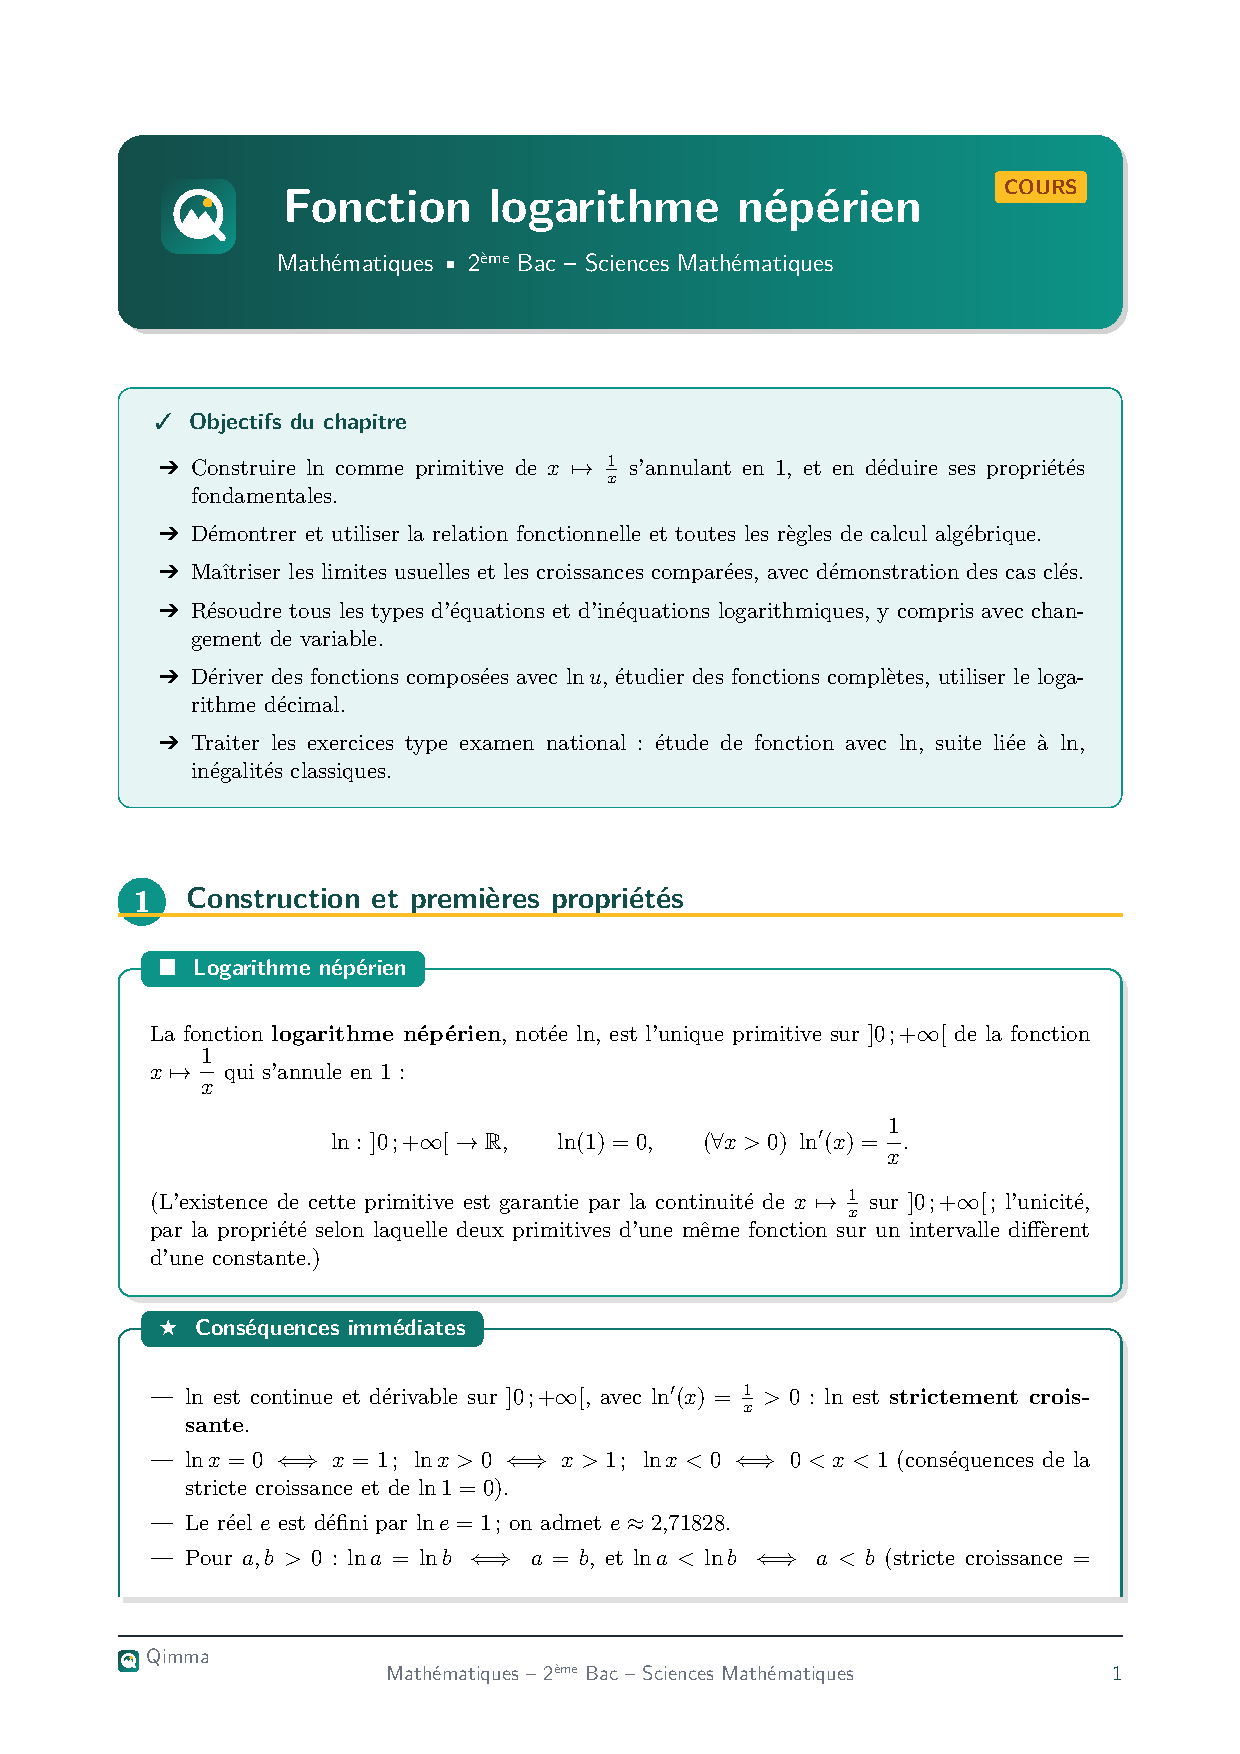
\includepdf[pages=-]{04-fonction-logarithme-neperien.pdf}
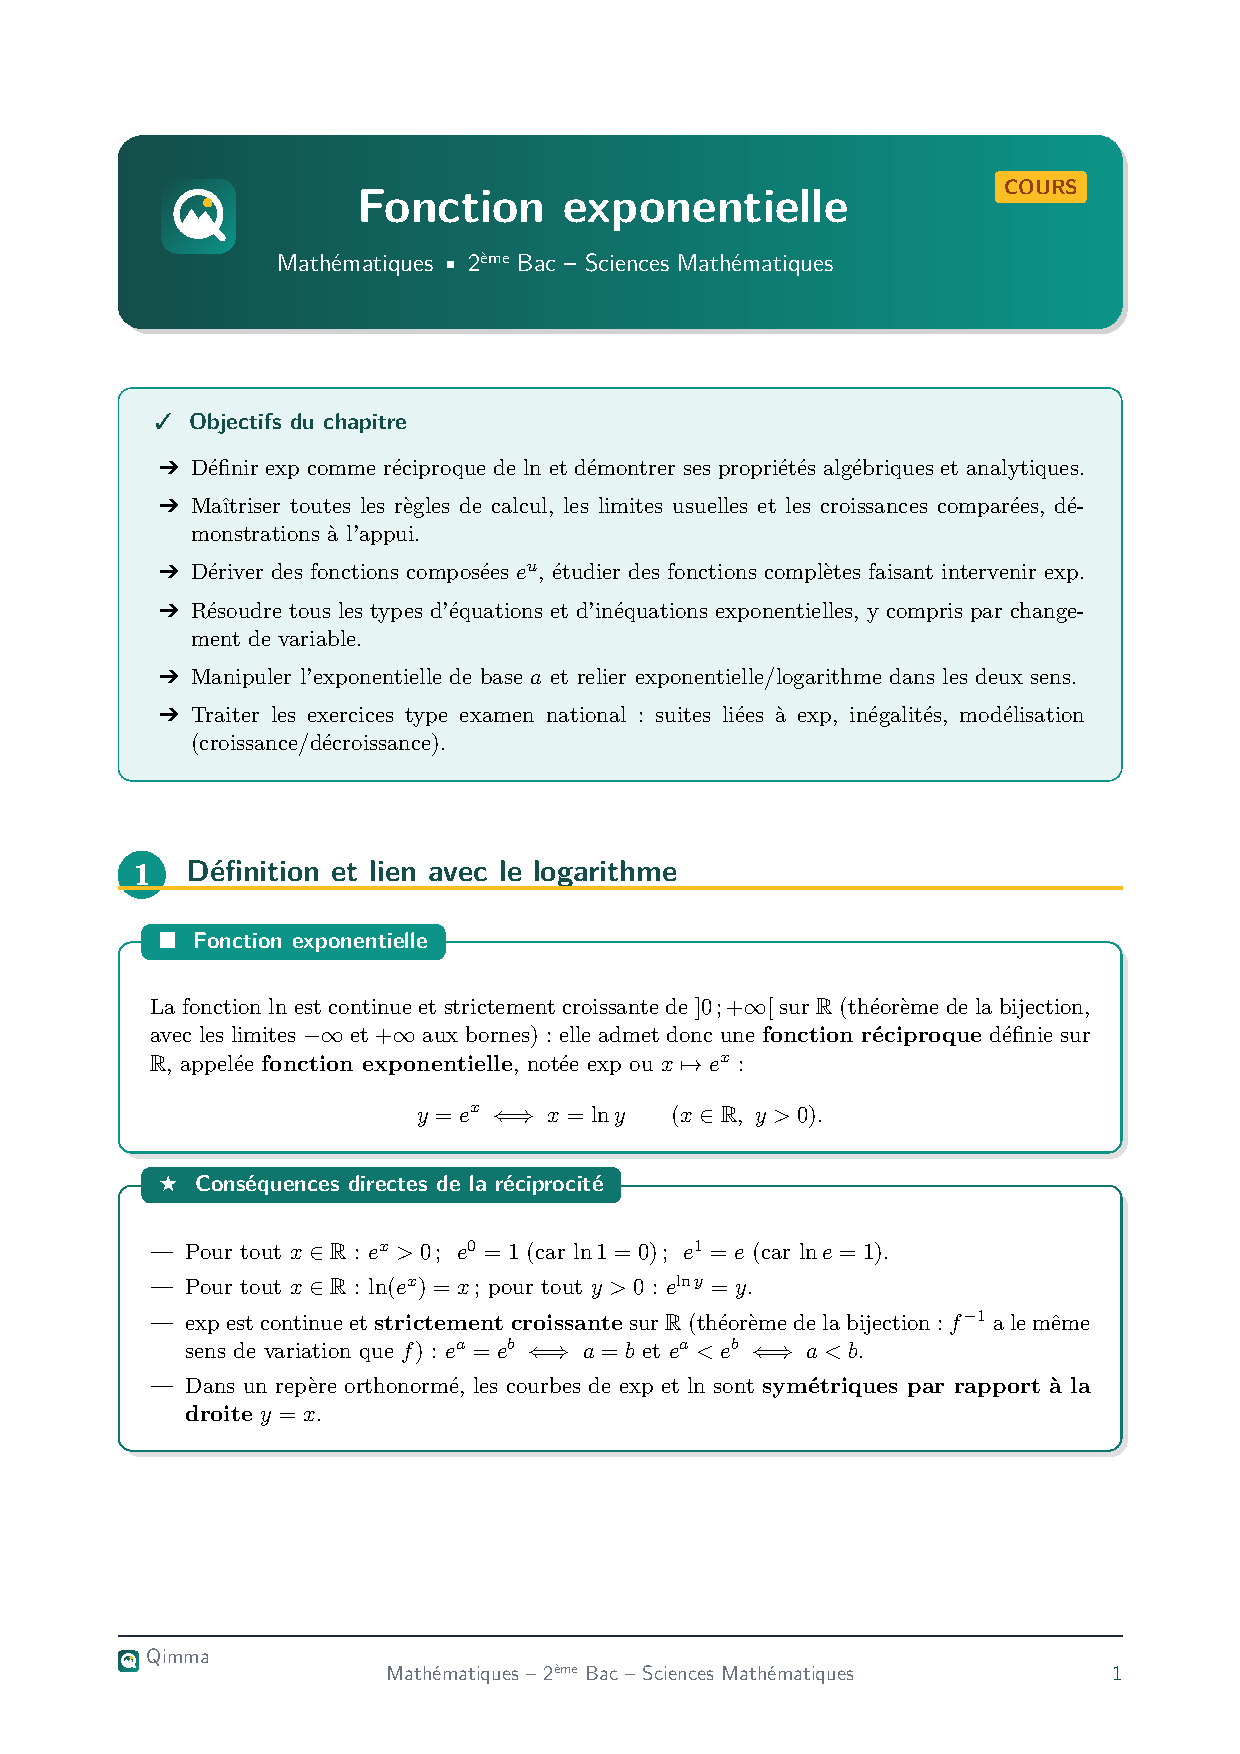
\includepdf[pages=-]{05-fonction-exponentielle.pdf}
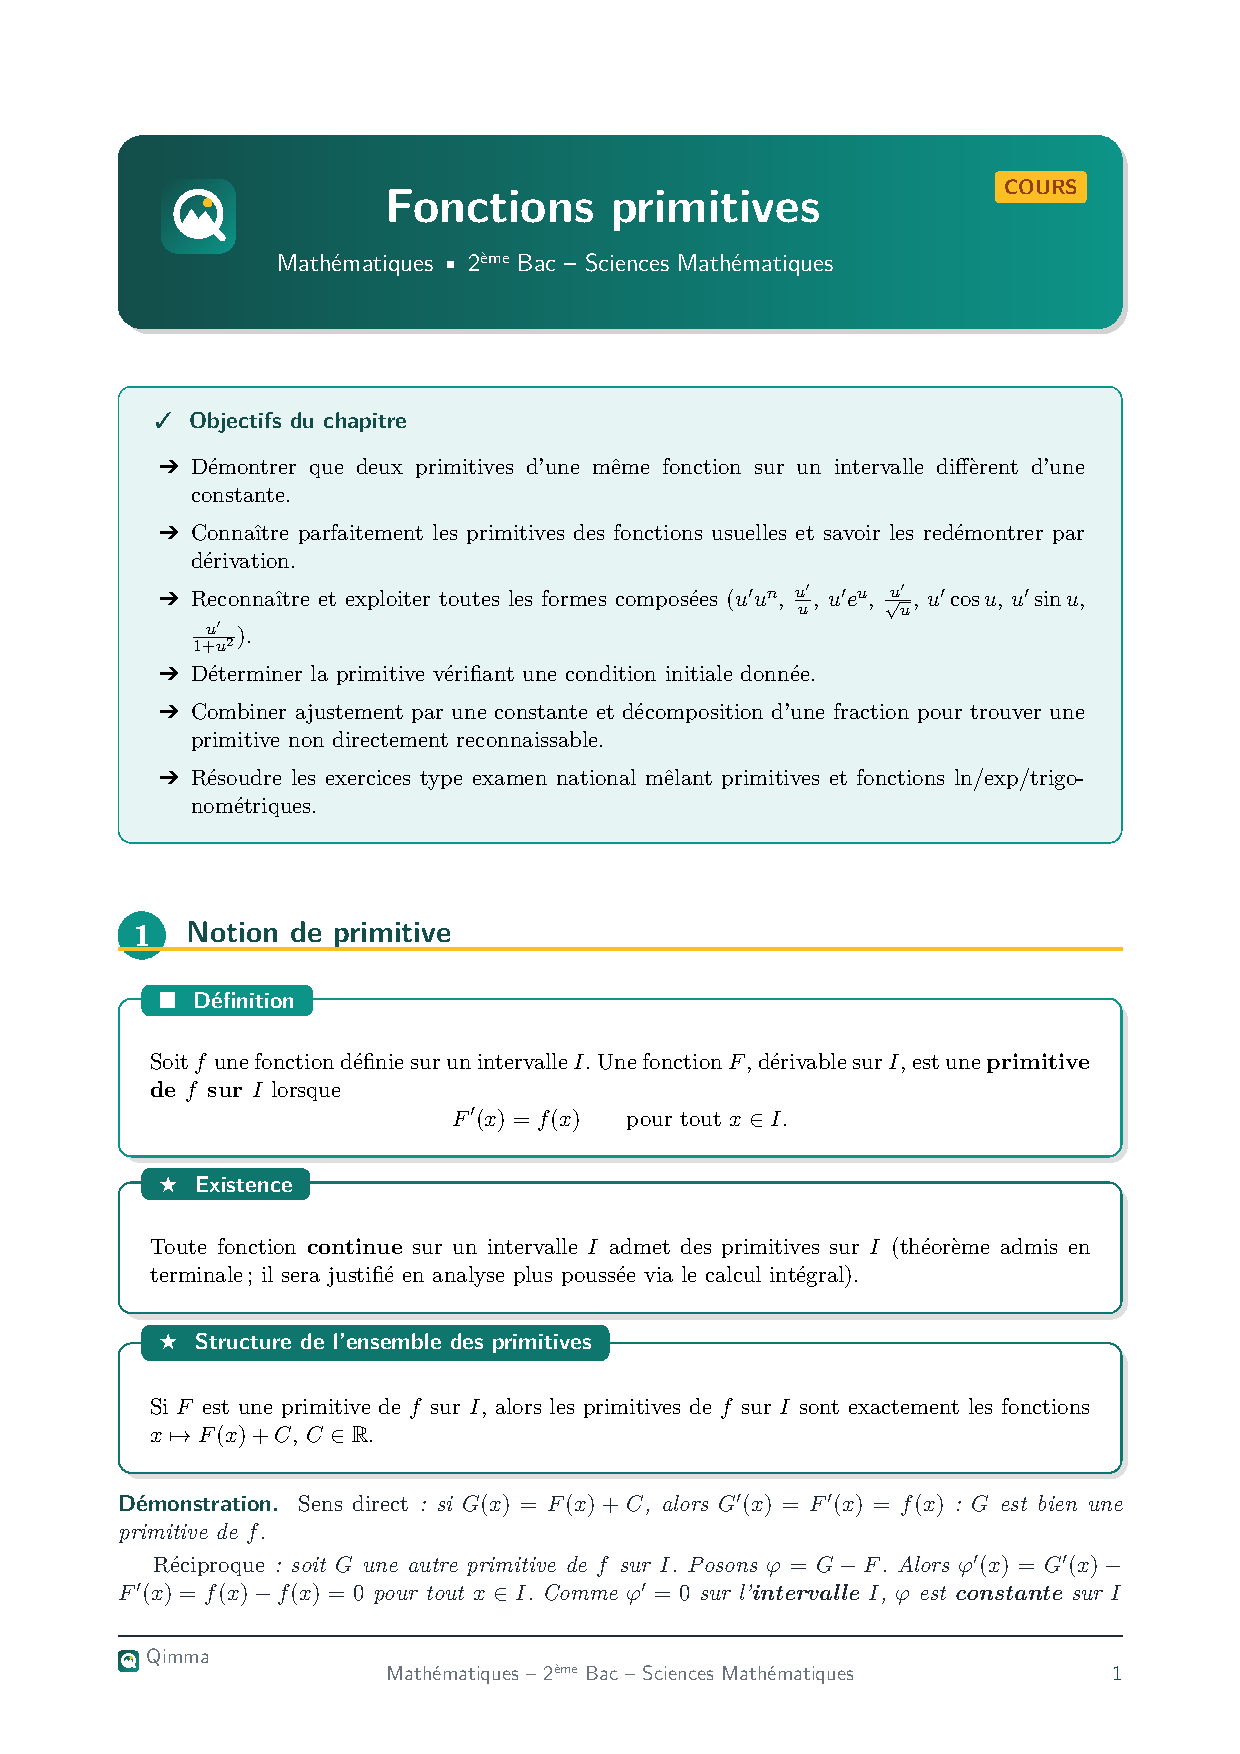
\includepdf[pages=-]{06-fonctions-primitives.pdf}
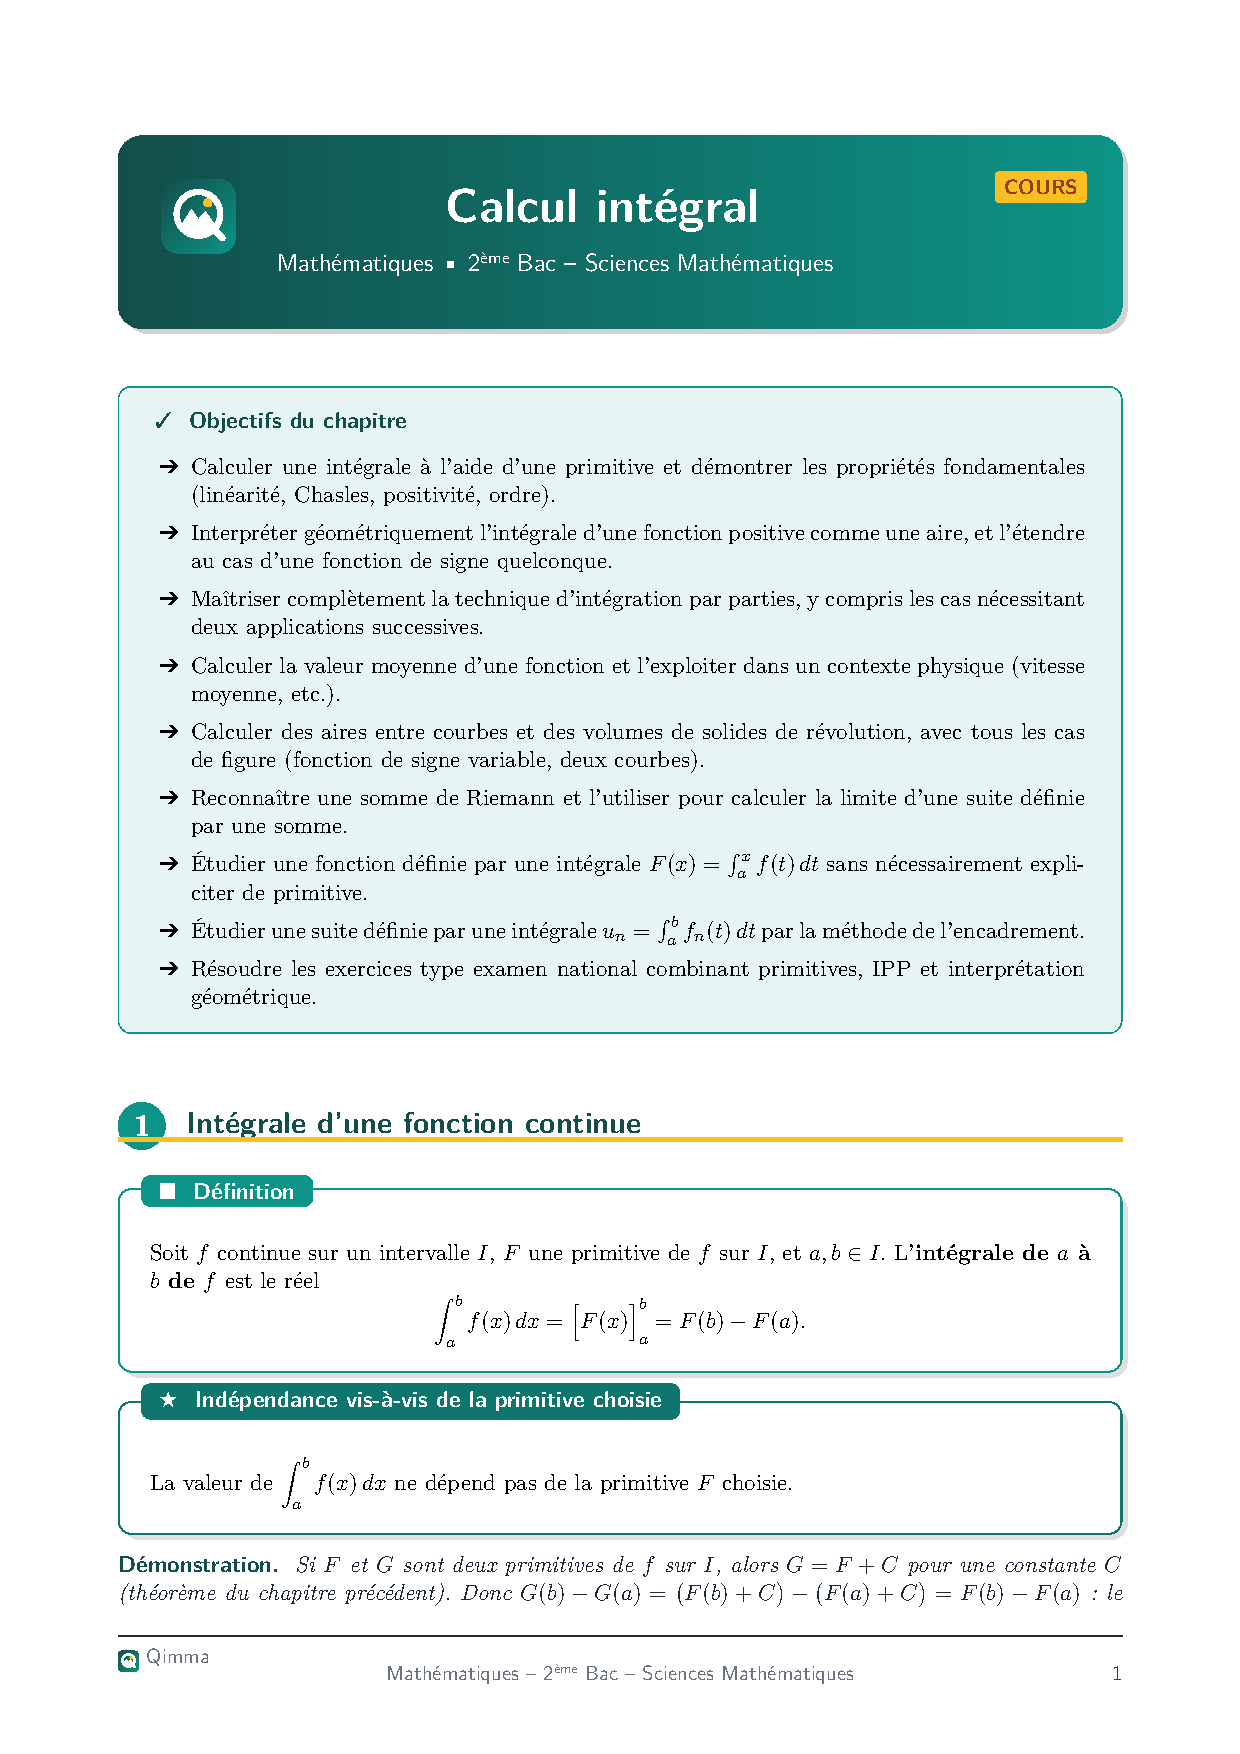
\includepdf[pages=-]{07-calcul-integral.pdf}
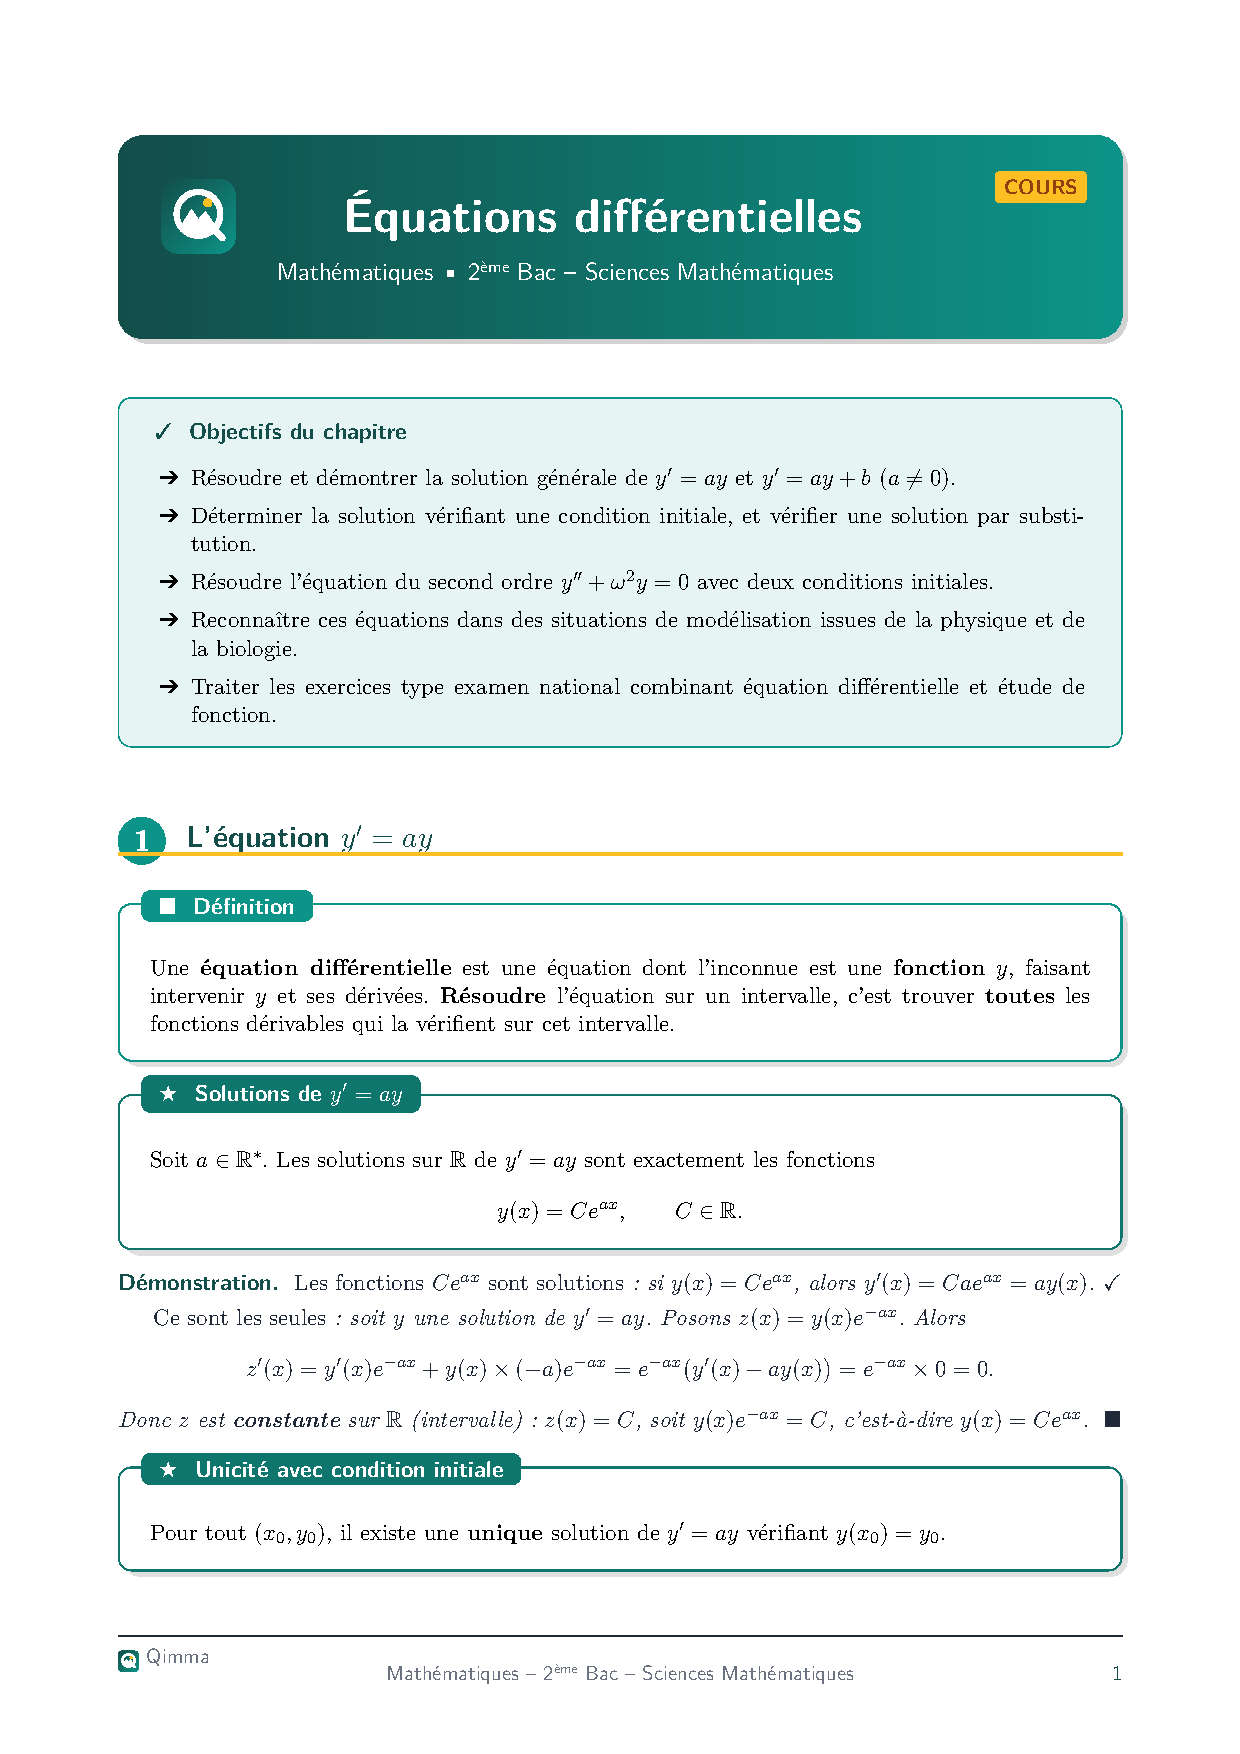
\includepdf[pages=-]{08-equations-differentielles.pdf}
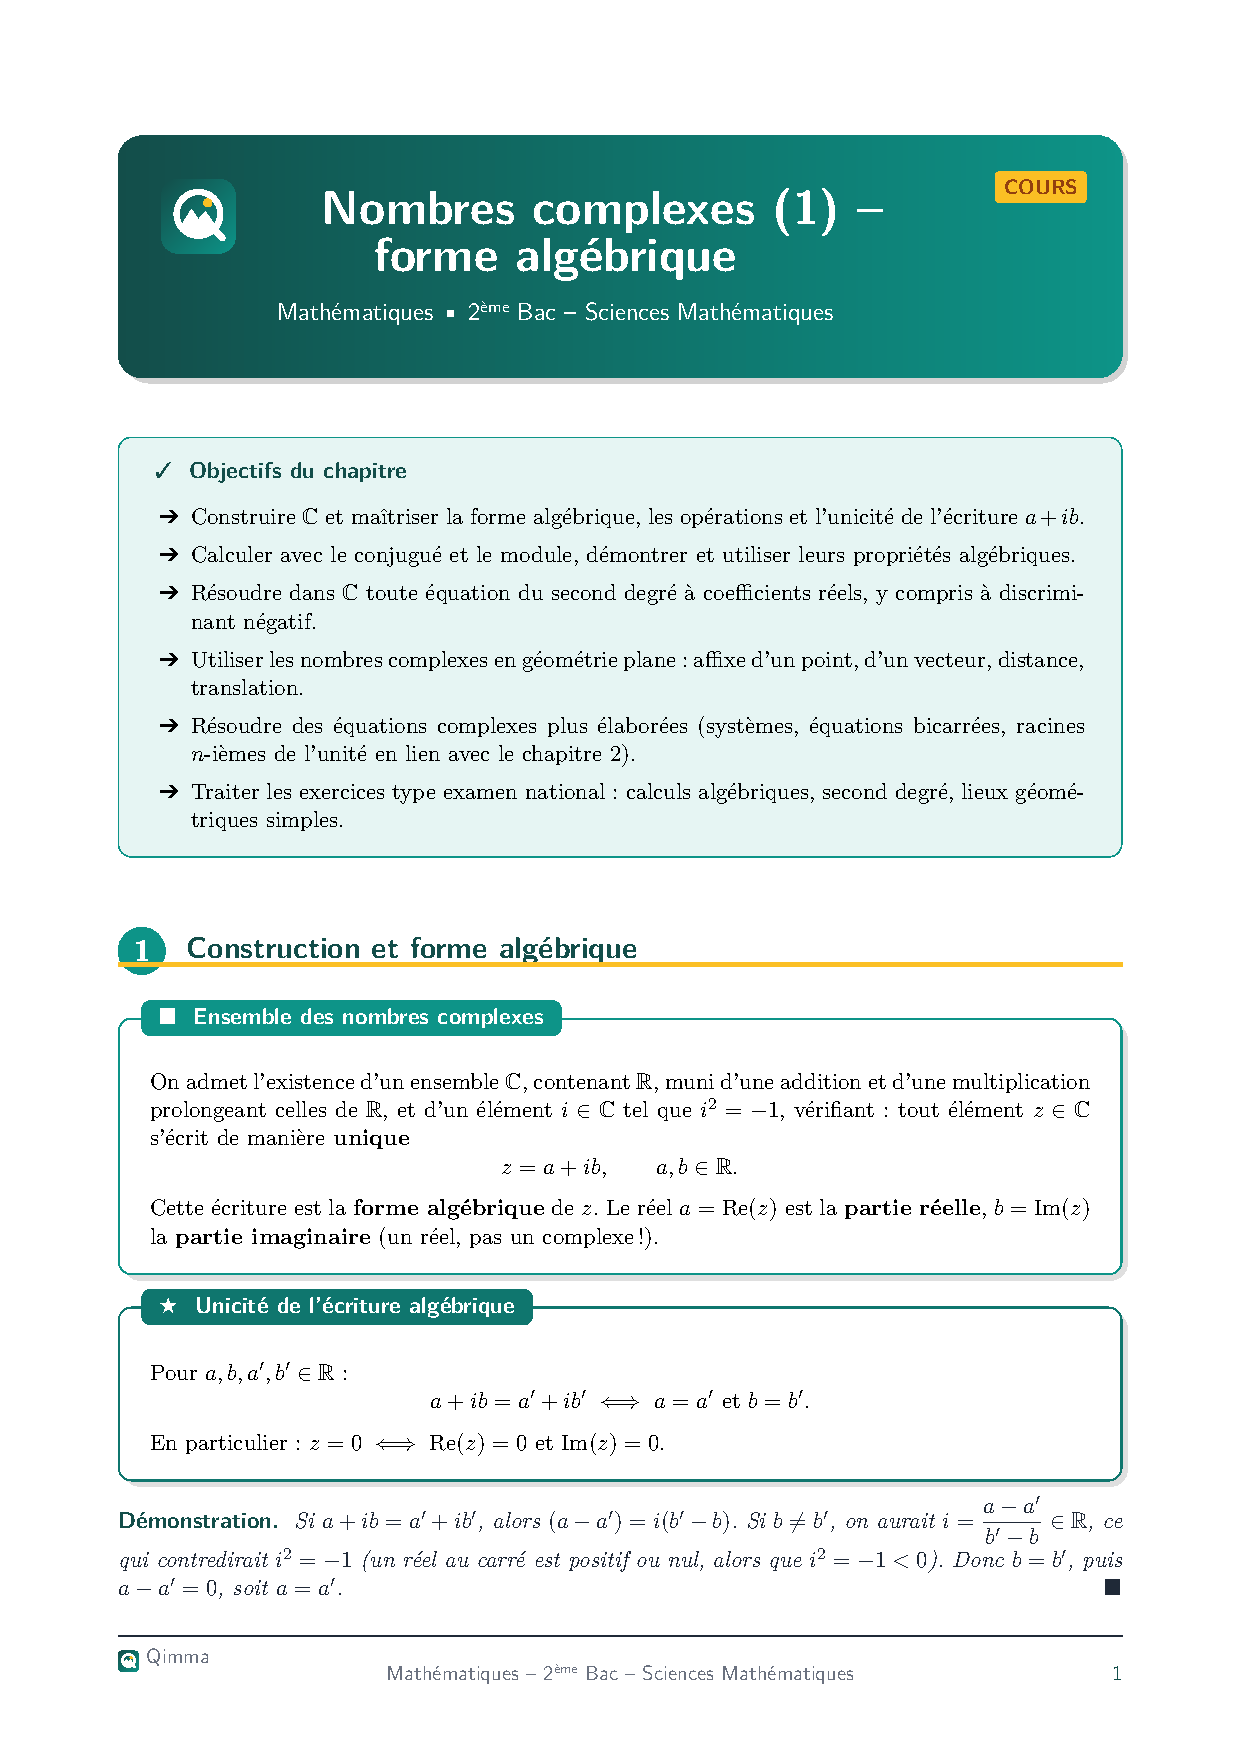
\includepdf[pages=-]{09-nombres-complexes-1.pdf}
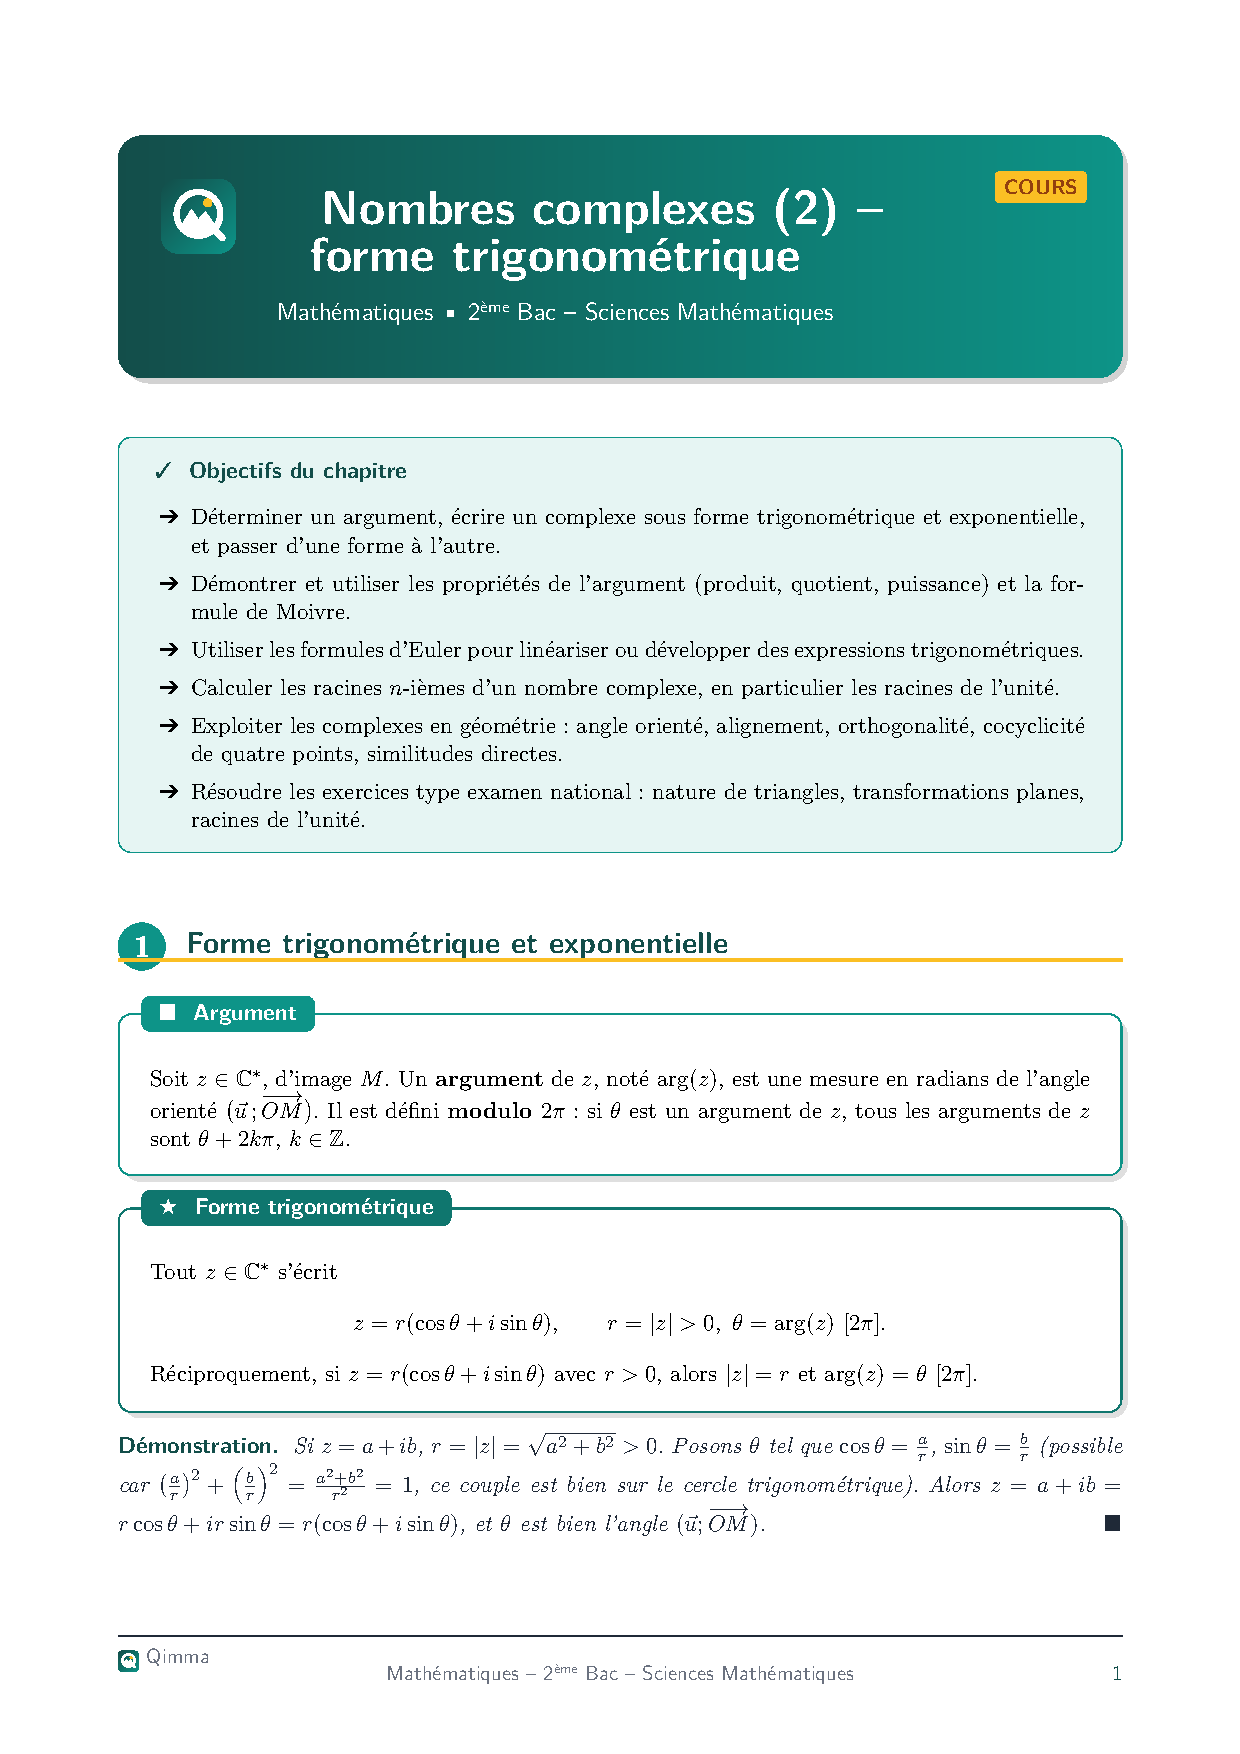
\includepdf[pages=-]{10-nombres-complexes-2.pdf}
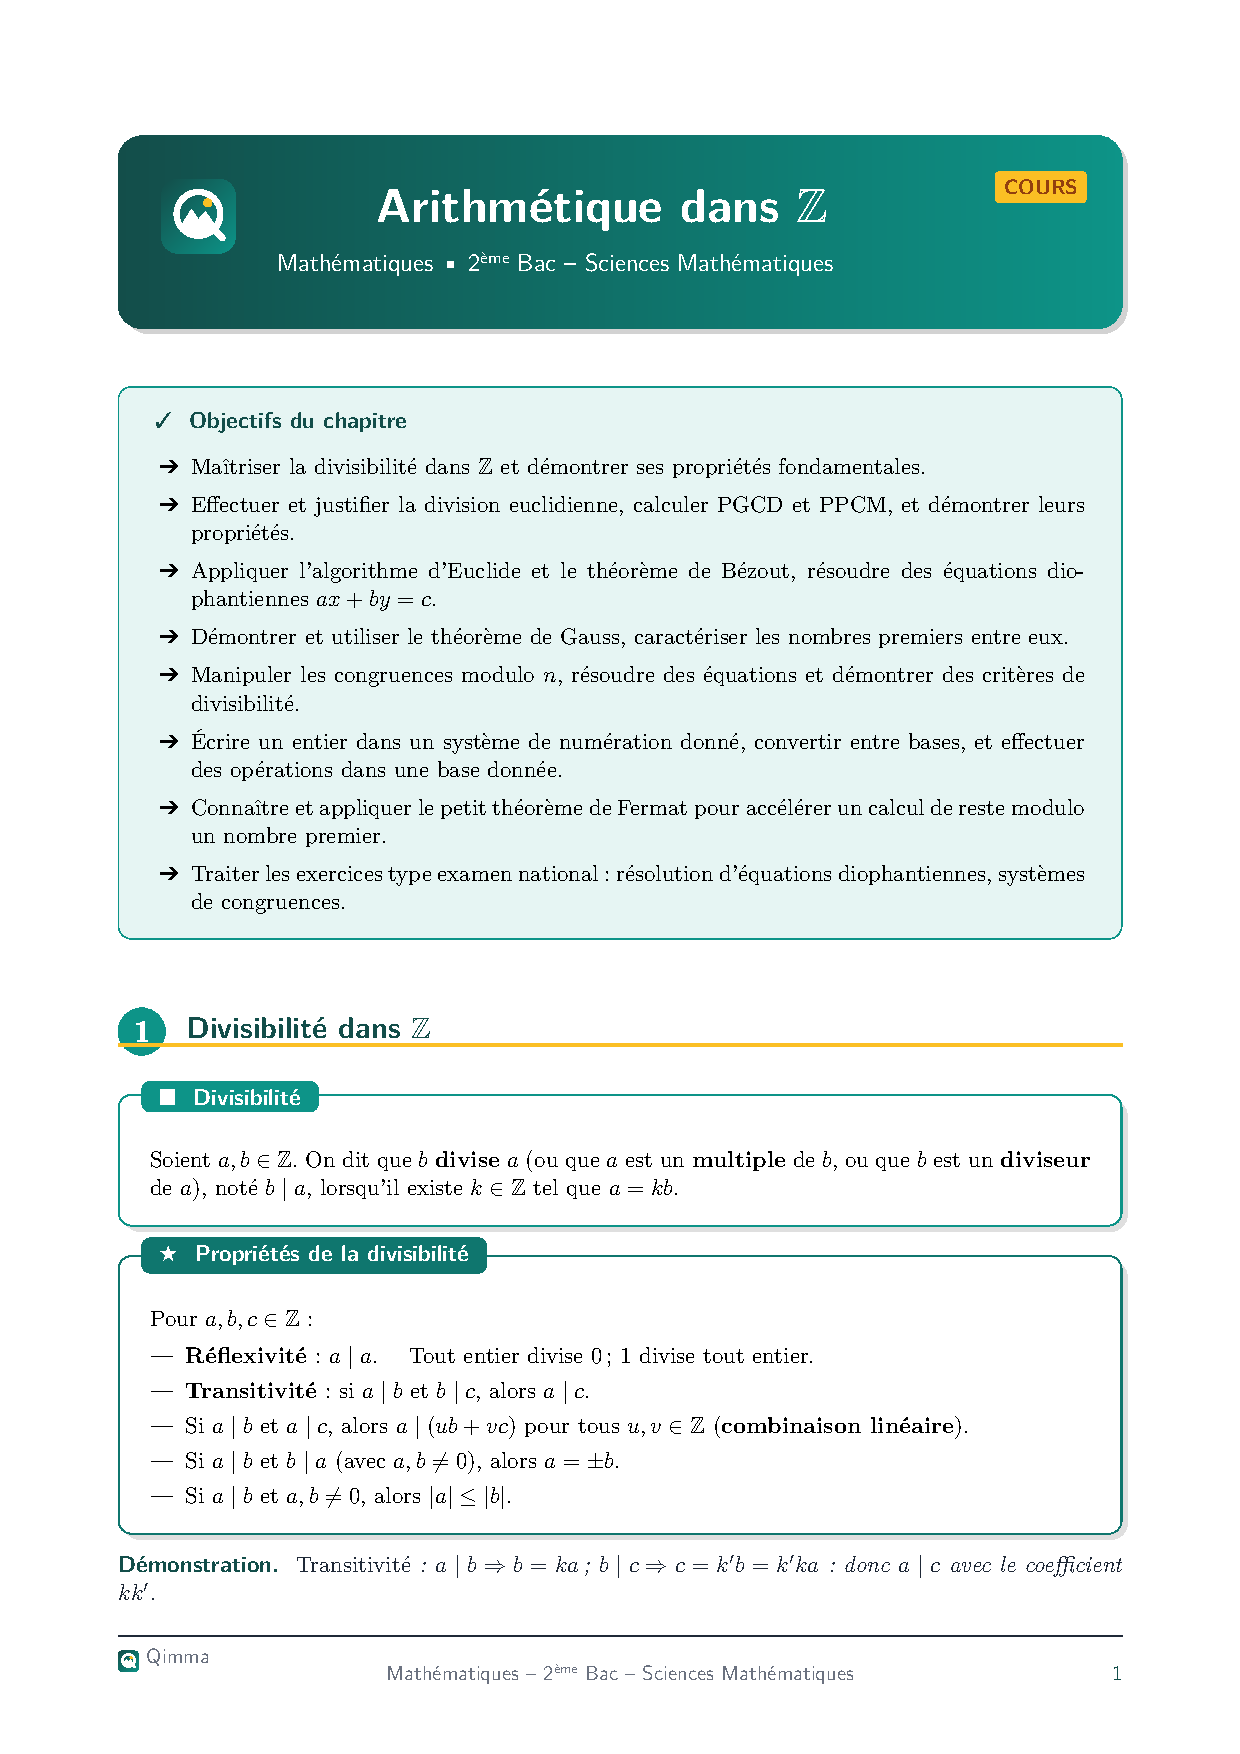
\includepdf[pages=-]{11-arithmetique-dans-z.pdf}
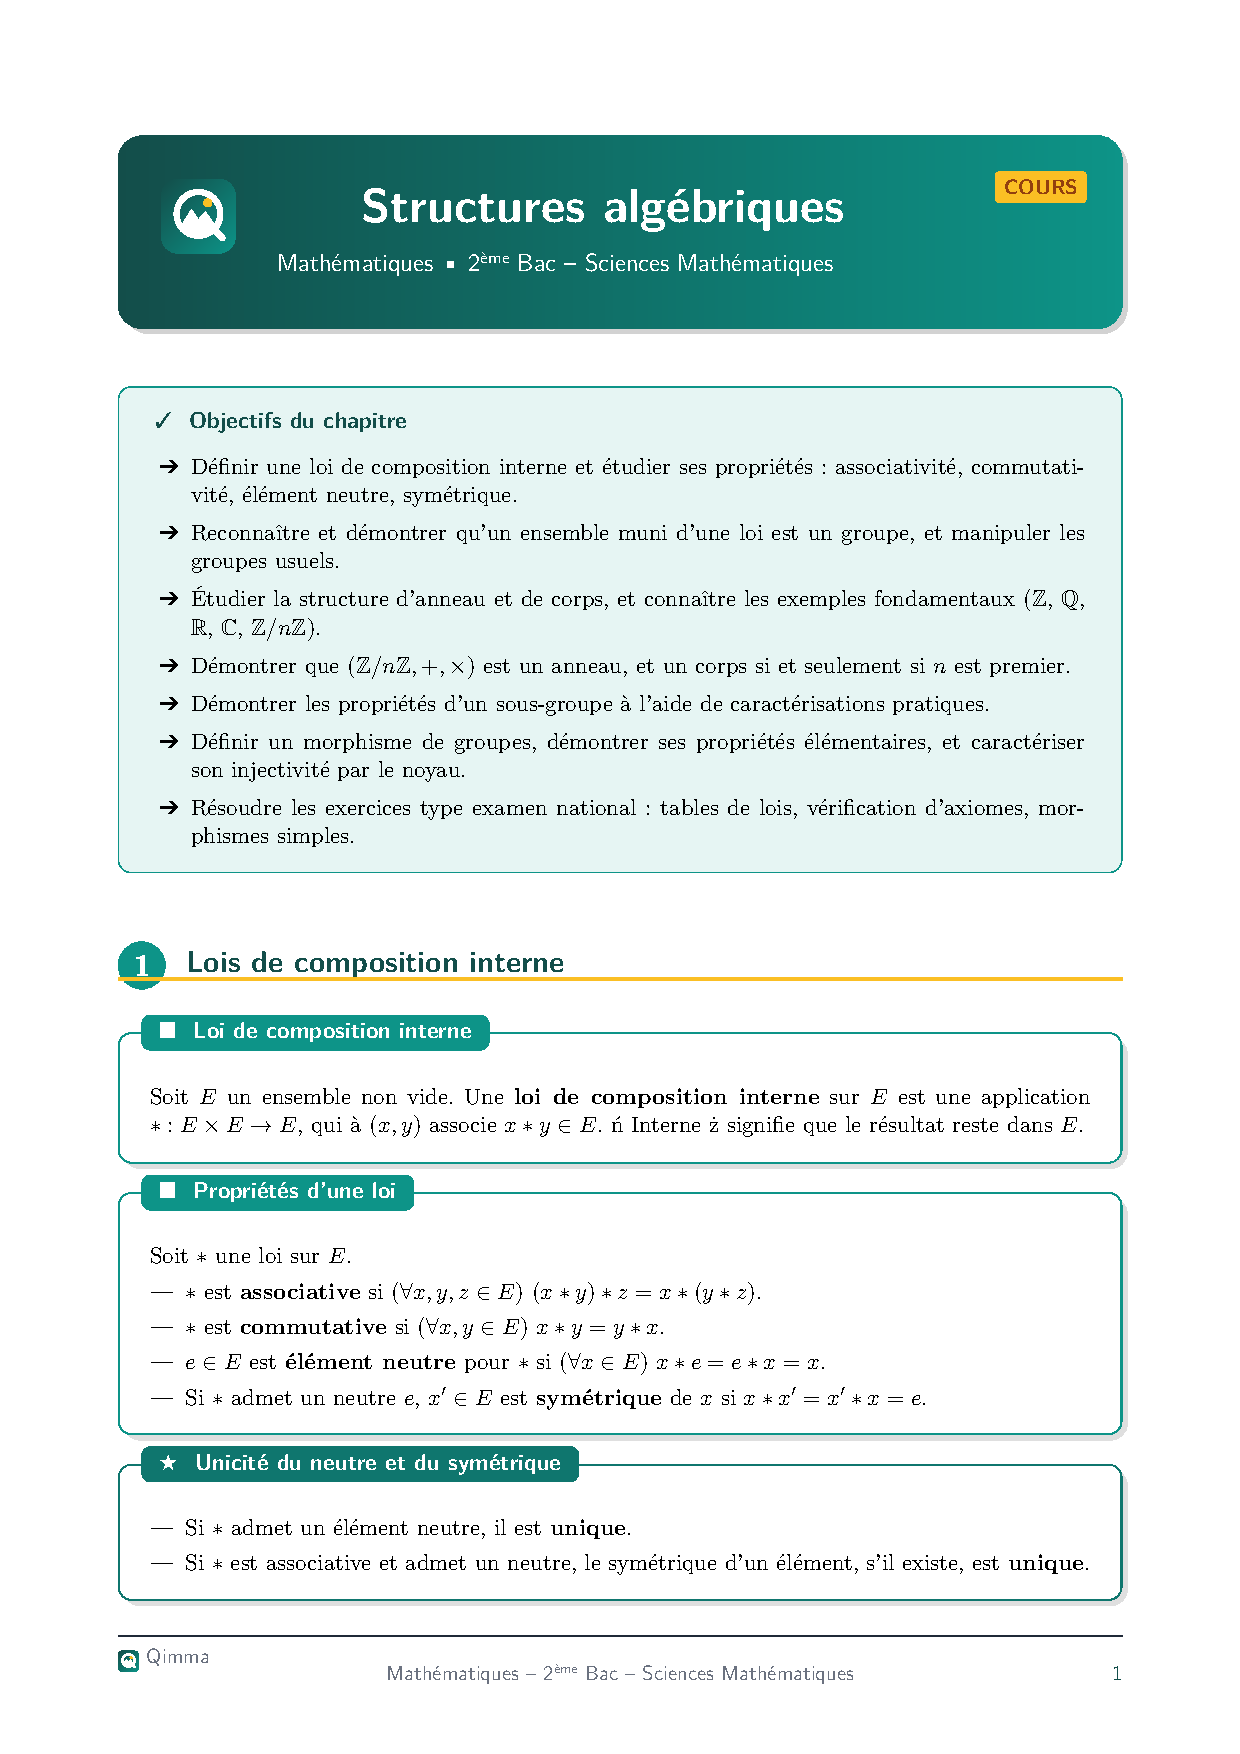
\includepdf[pages=-]{12-structures-algebriques.pdf}
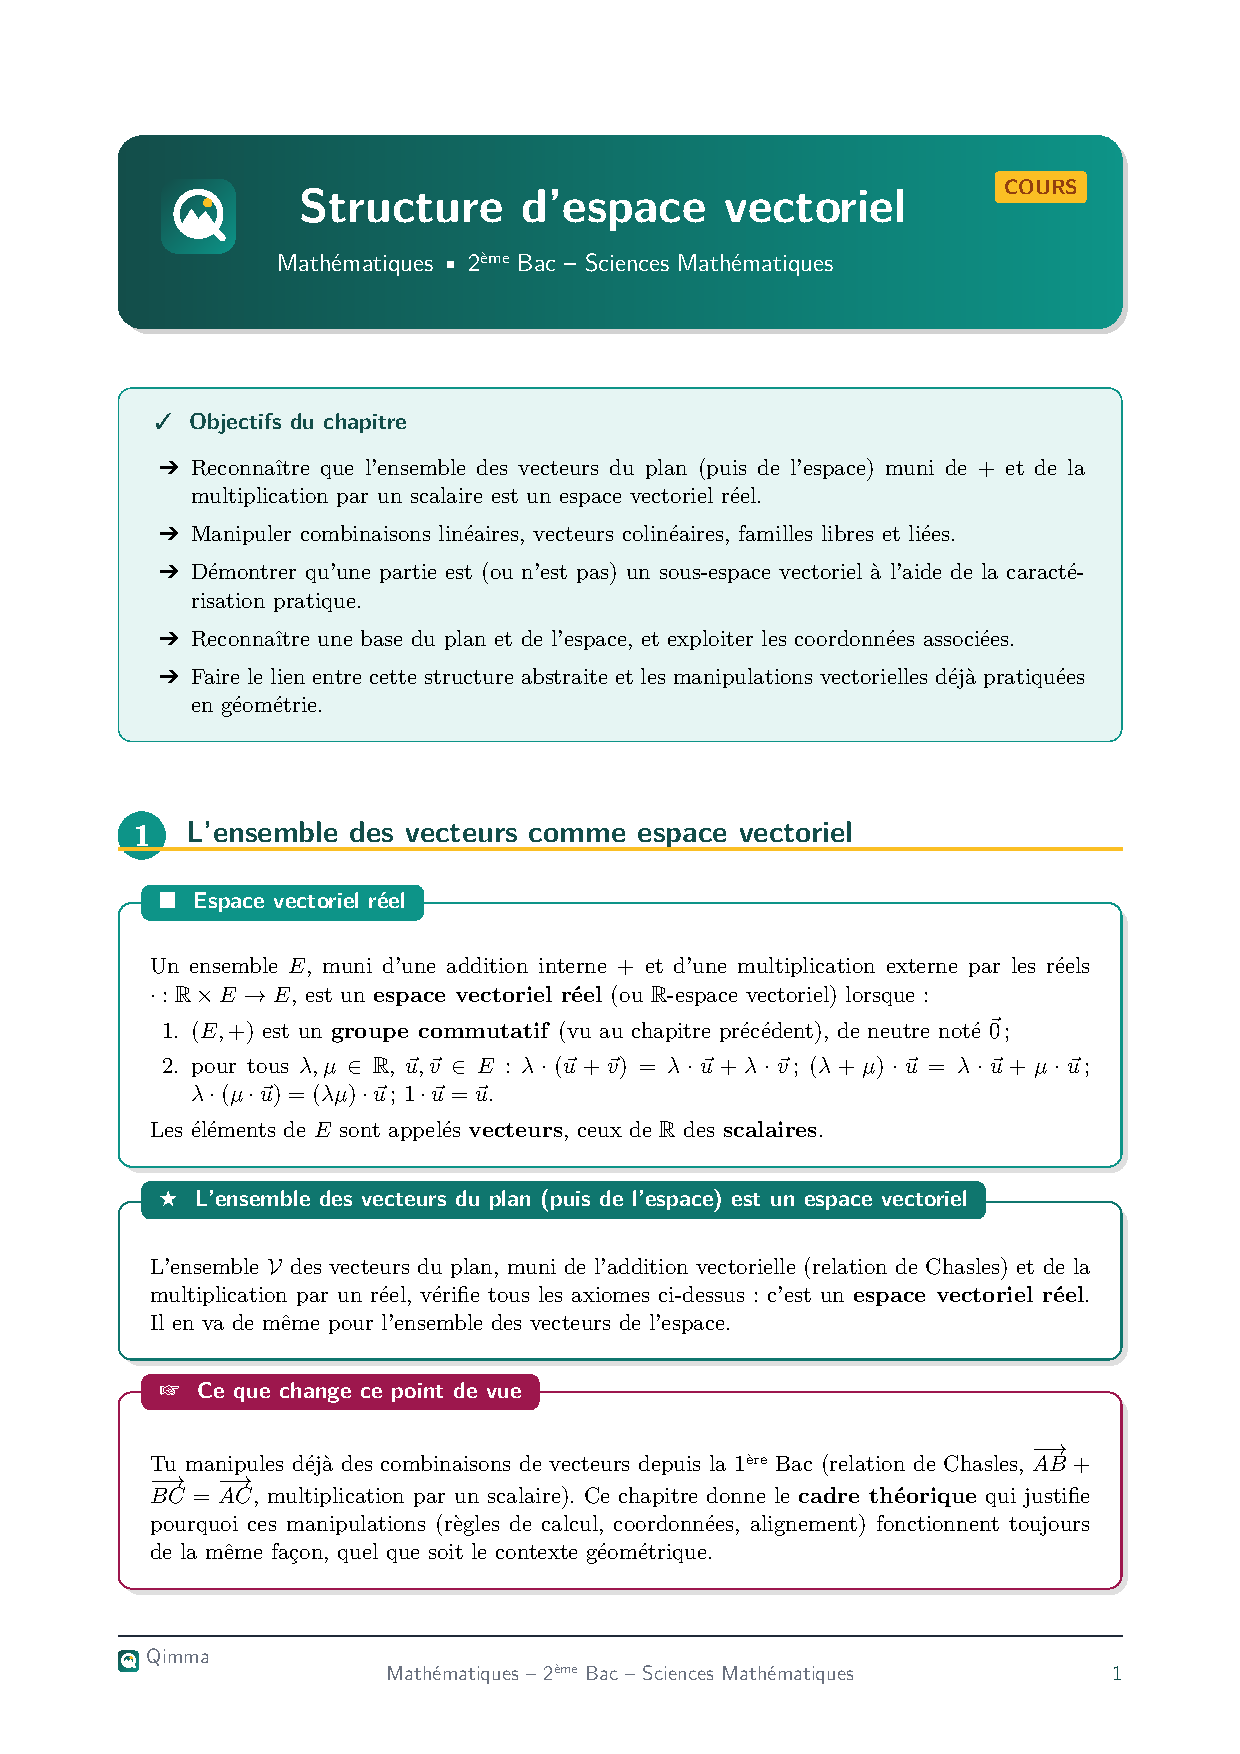
\includepdf[pages=-]{13-espaces-vectoriels.pdf}
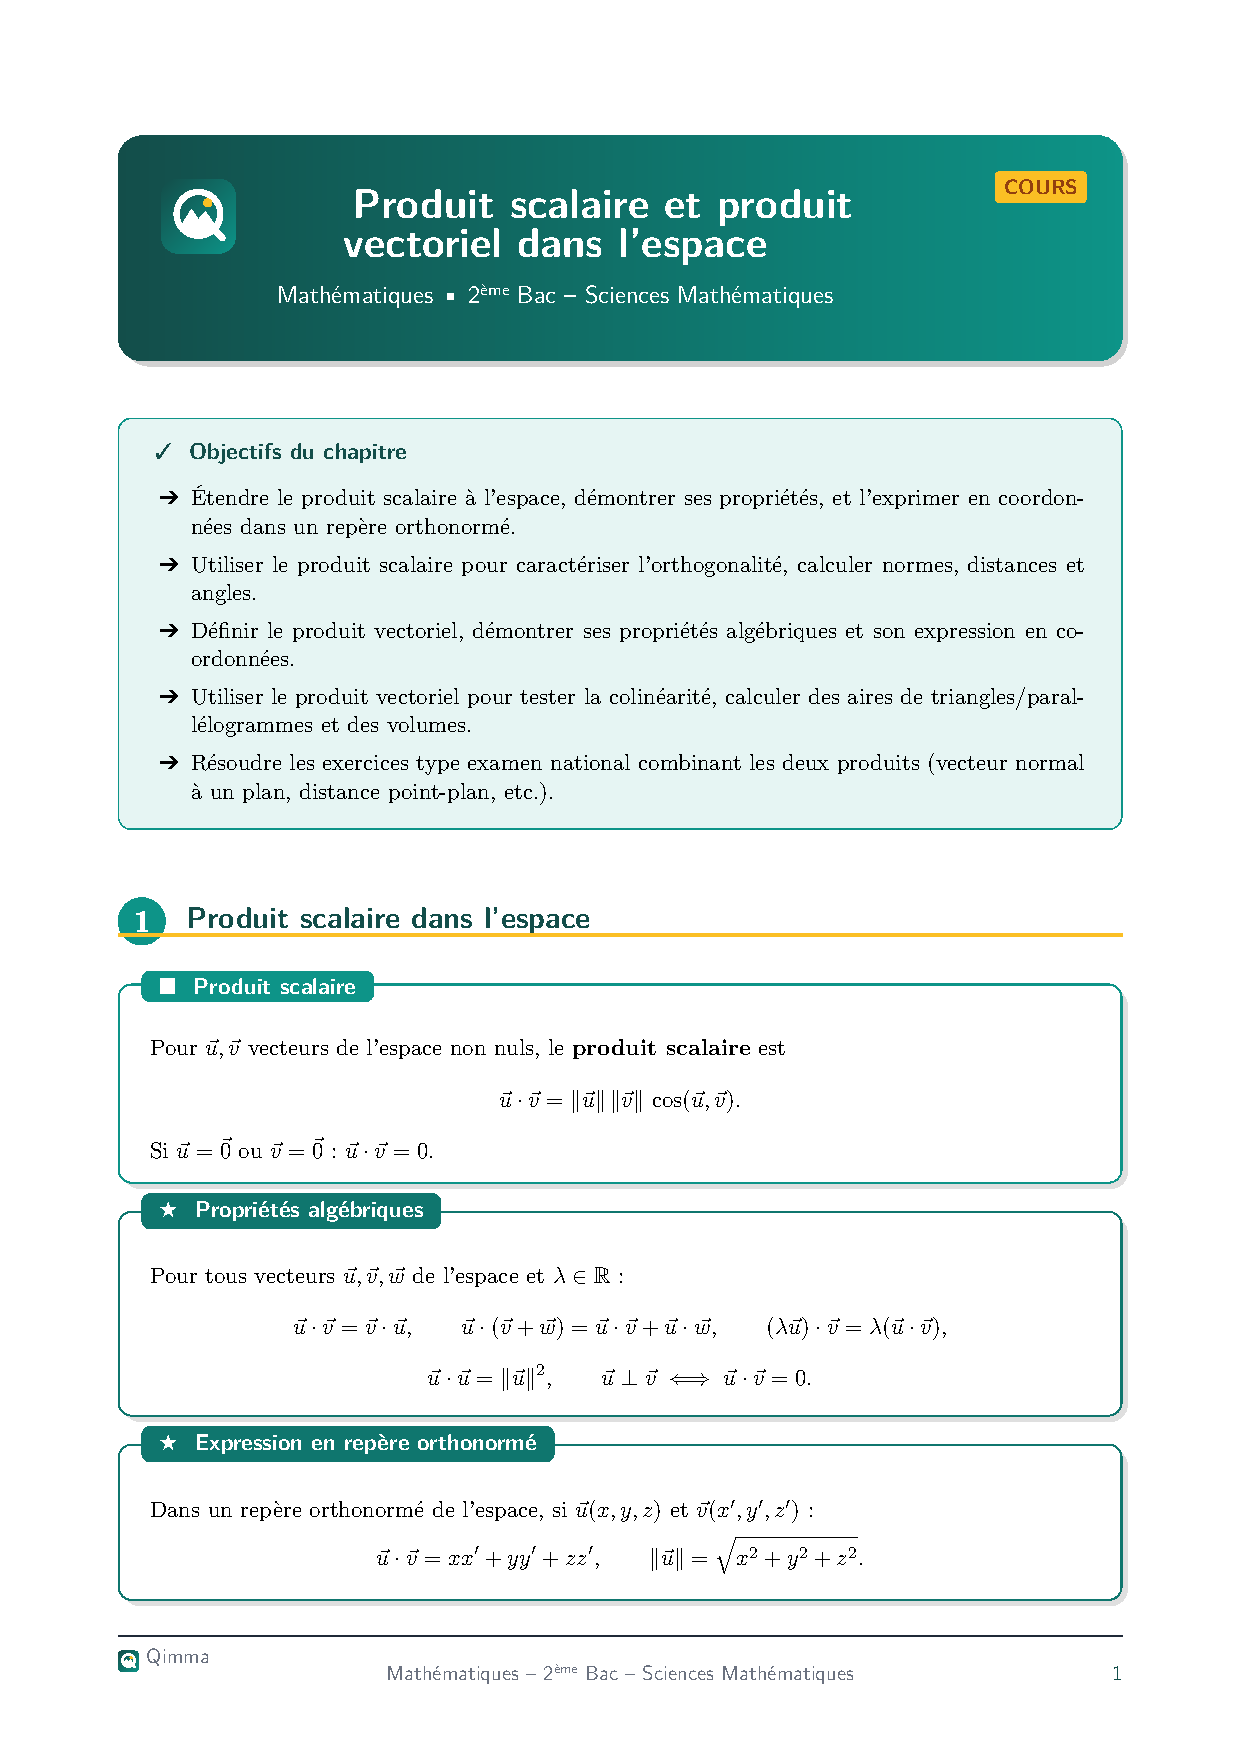
\includepdf[pages=-]{14-produit-scalaire-vectoriel-espace.pdf}
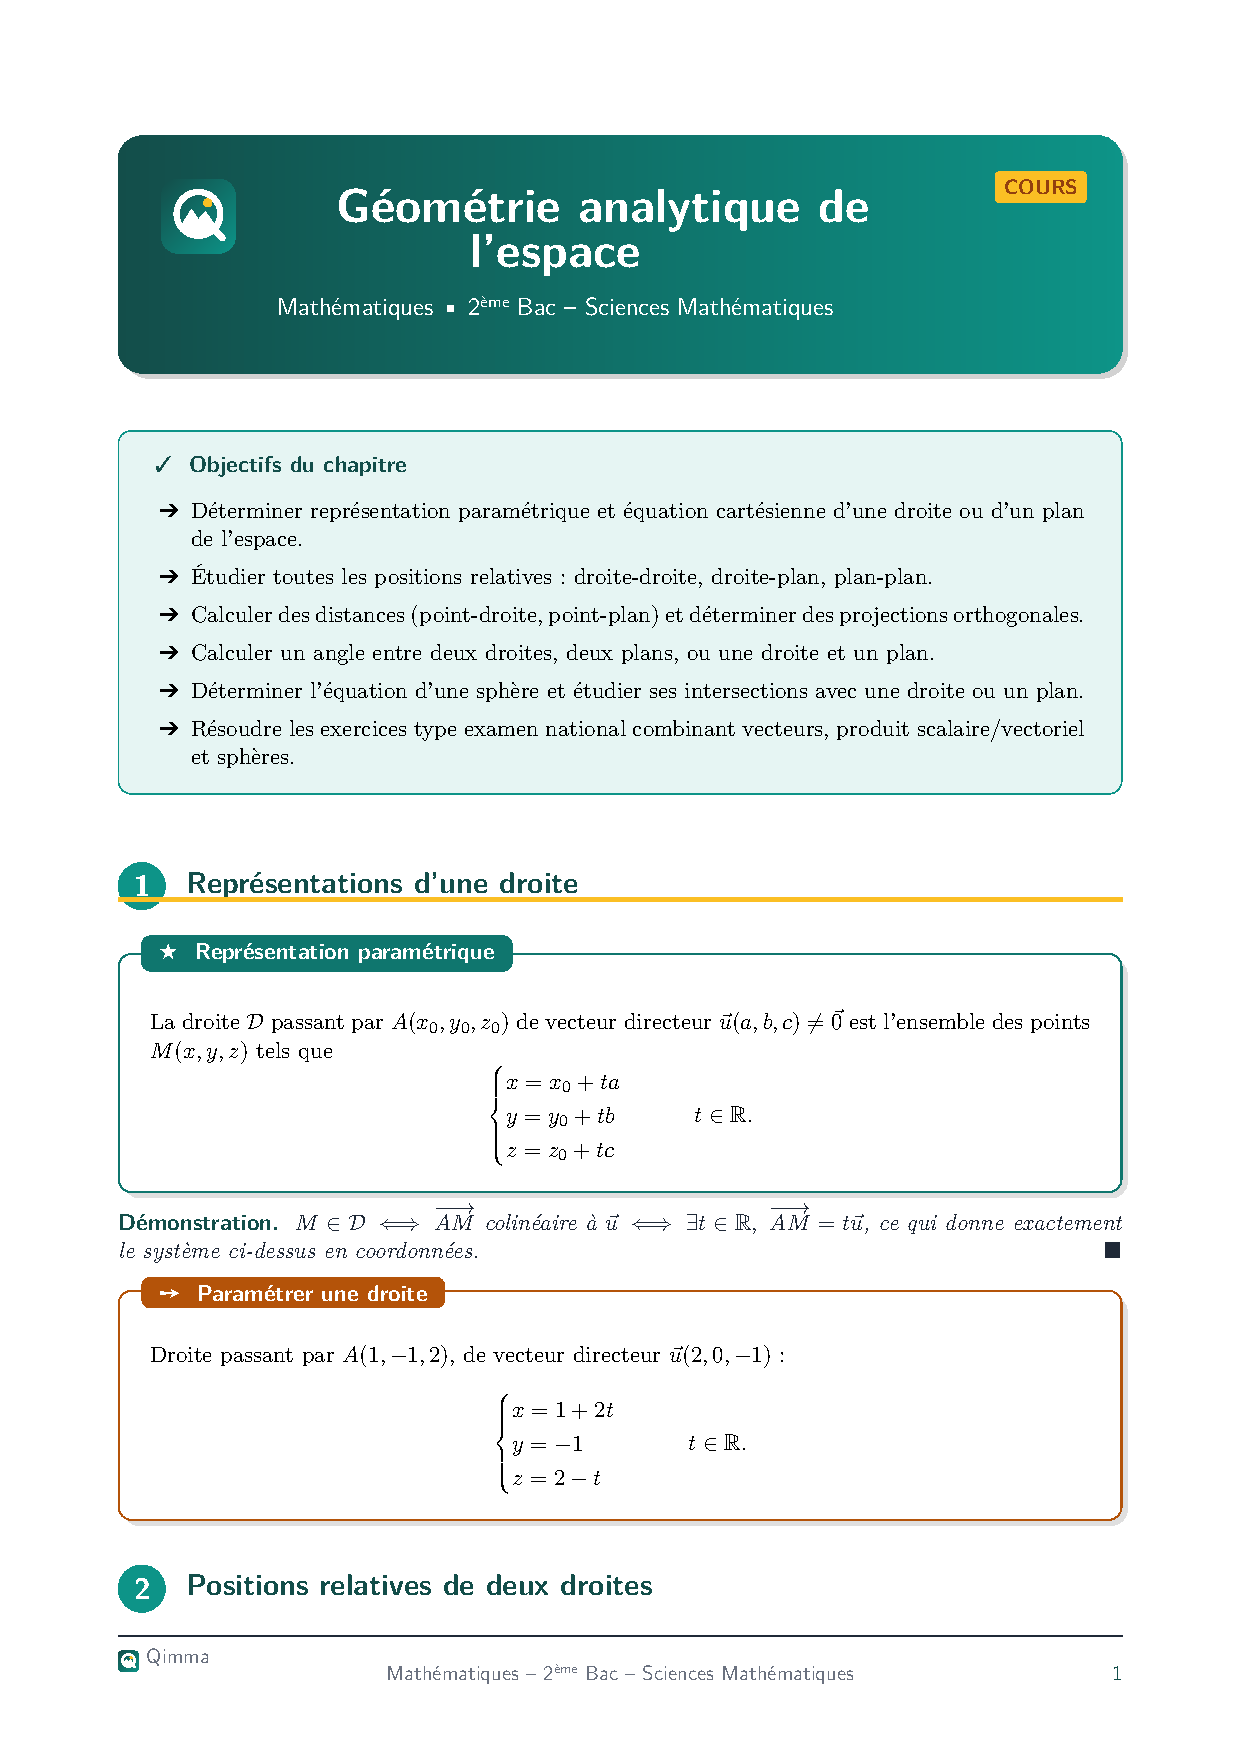
\includepdf[pages=-]{15-geometrie-analytique-espace.pdf}
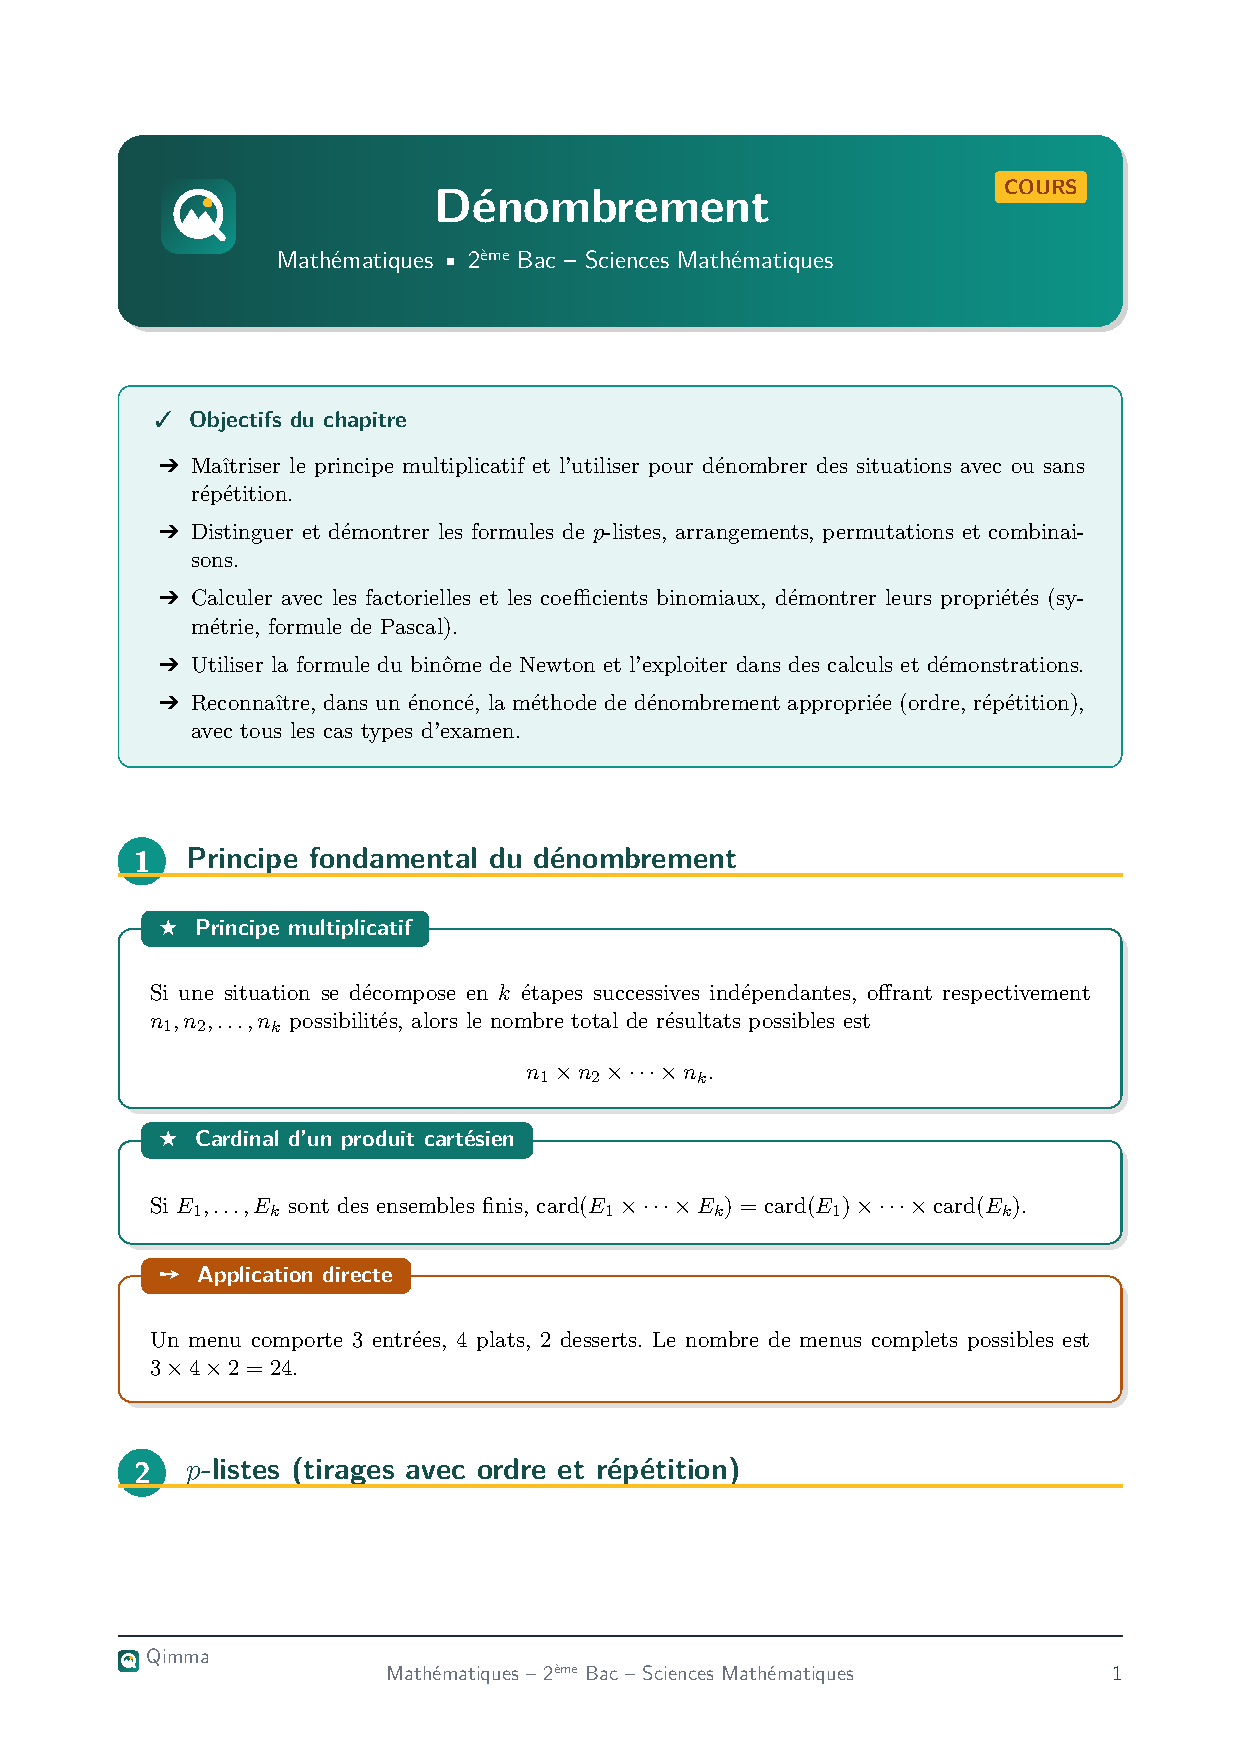
\includepdf[pages=-]{16-denombrement.pdf}
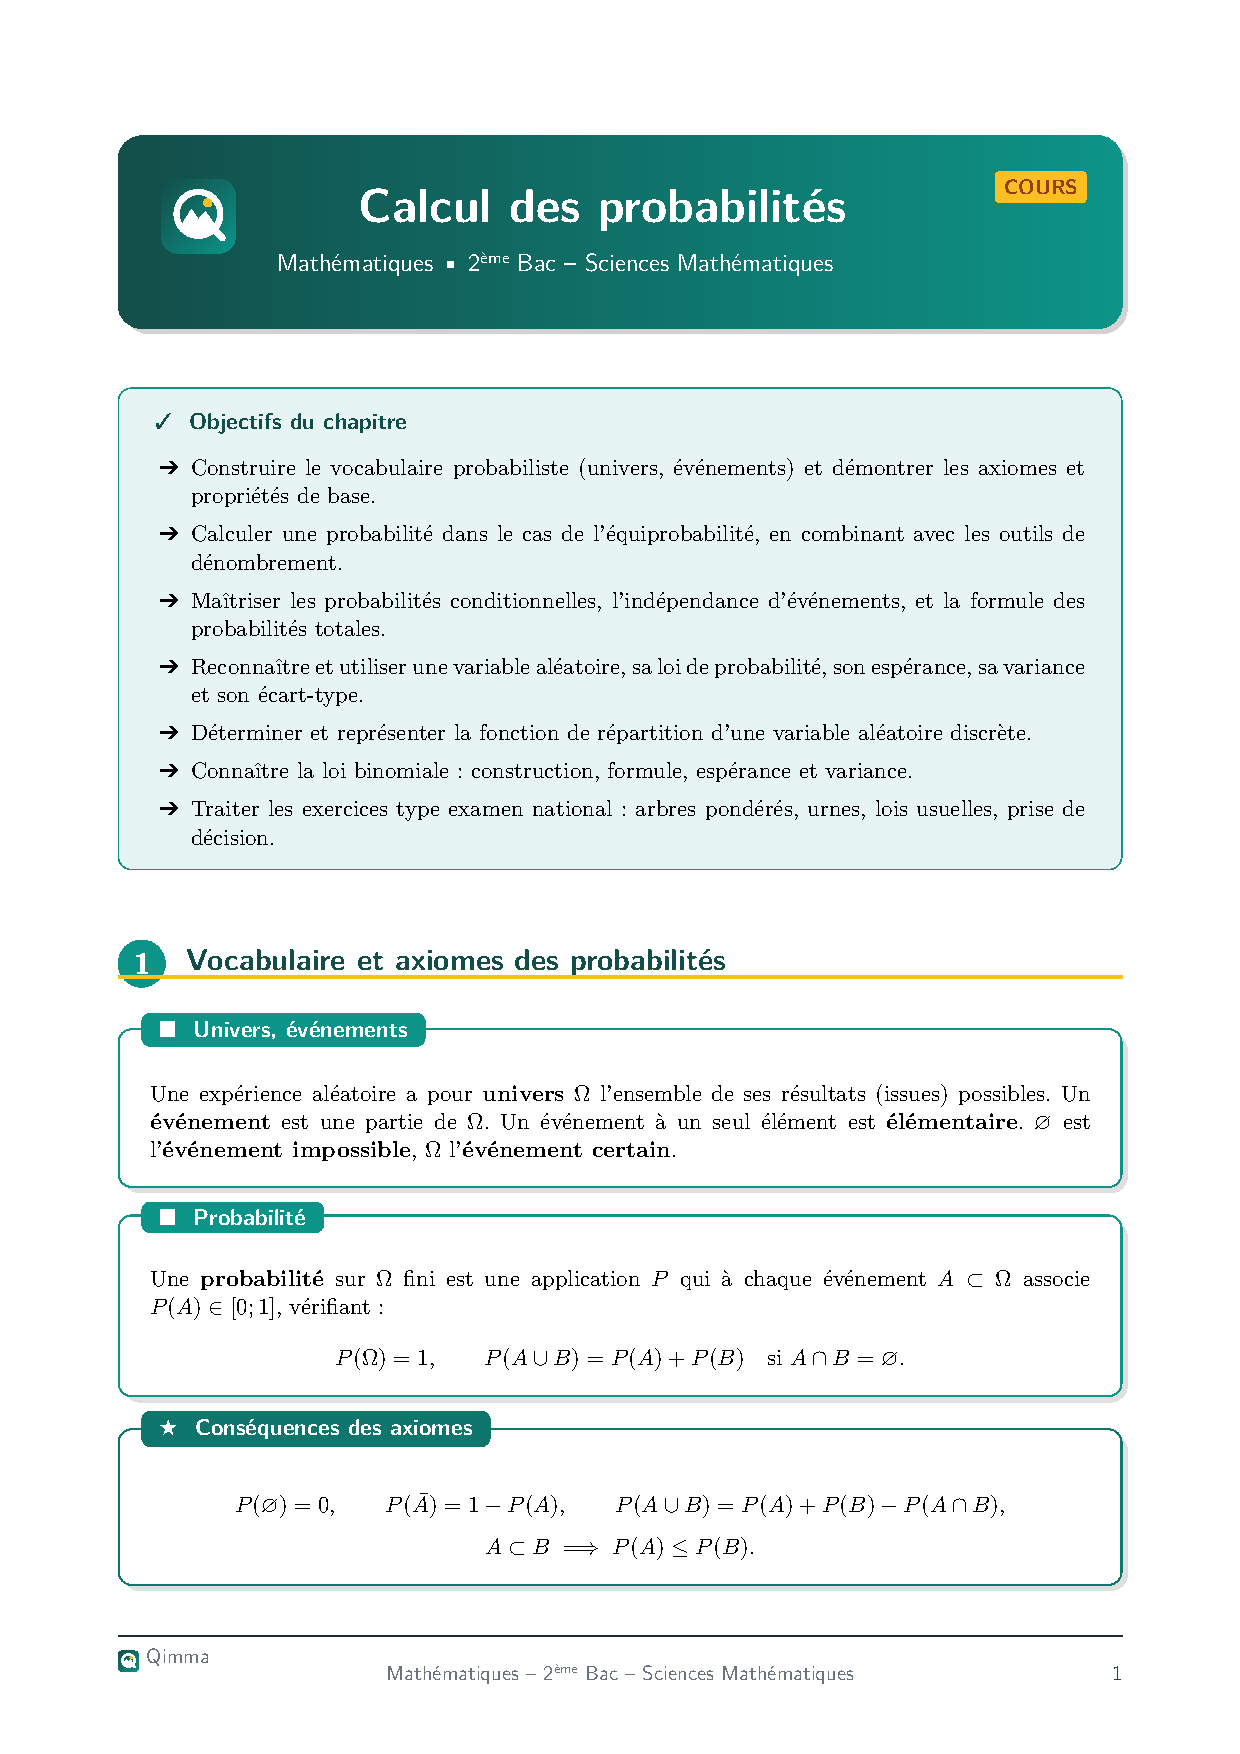
\includepdf[pages=-]{17-probabilites.pdf}

\end{document}
